% Chapte 7
\chapter{Advertisement application} % Main chapter title

\label{Chapter7} % For referencing the chapter elsewhere, use \ref{Chapter1} 
\newpage

\section{Introduction}
The use of technology in advertisement plays a major role in advertisement industries. It would have been much difficult to reach to customers without technologies, and technology enhances the two-way communication with the client and the customers. The companies can now easily express their thoughts and vision to their customers with the help of the latest technologies. Advertisements are everywhere, in websites, in your smartphone, in television and radio. Since the last decade, it is more common to see advertisements on the streets, in supermarkets, airports and any place of public gatherings.
So, for every context or settings there are different kinds of technology that are being used to make the advertisement more appropriate. When it comes to interactive advertisement, the use of right technology plays another major role in terms of usability and understandability. Interactive advertisements on websites are usually interactive using keyboard and mouse, whereas in smartphone, advertisements use only the capability of the touch or other sensors to make the interaction easy. Interactive advertisements in public spaces have another bunch of technologies that make the interaction usable like using face recognition, body position recognition, hand gesture recognition and also touch sensors, proximity sensors and much more.


This chapter explains all the technical aspects of the advertisements system that were developed during the thesis work for attracting attention and the main advertisement application. It discusses what technologies and hardware have been used and what algorithm and methods were implemented to accomplish the goals. Besides the technical details it describes the interaction design of interactive advertisement.



\iffalse
\section{Attracting attention Application}
The goal of attraction attention was to develop systems that could attract the attention of the passers-by, in which three different applications were developed and later compared.

\subsection{Requirement gathering}
The below are the required elements used for the applications.


\subsubsection{Hardware requirement}

\begin{itemize}
\item \textbf{Microsoft Kinect Camera} \cite{Kinect} \\
This is one of the most used camera in public context a lot, this camera can track up to seven user's position (X, Y, Z) in real time; it is capable of recognizing hand gesture and even can track facial movements. The camera does not work well when it is exposed in sunlight, which makes it ideal for indoor use only. In our experiment Microsoft Xbox 360 Kinect camera was used, The Kinect camera should be used with an extra adapter in order to connect it to computer. 
\item \textbf{Computer} \\
A normal laptop was used with Core i7 2.7 Ghz processor, and 4 GB RAM and USB of 2.0 version.
If you want to use Xbox Kinect One Kinect then the computer should support USB version 3.0.
The laptop was connected to the University monitor via mini display port.

\end{itemize}


\subsubsection{Software requirement}
The software can run in any operating system except because of the processing programming language. In experiment mac OSX operating system was used with below library and processing version.
\begin{itemize}
\item Processing v2.2.2 or higher version.
\item SimpleOpenNI library for Processing \cite{simpleopenni}
\item 32bit JRE (Java Runtime Environment) v1.8 or higher.
\end{itemize}


\subsection{Following eye application}
The name is given \emph{Following eye} because the application shows eyes for each individual when pass from the front of the screen and those eyes follow the person where they walk. The interaction works with the Kinect camera that provides each individual positions.
Explore the attached CD for the source code.

\subsection{Firework application}
This application also uses kinect camera to track user position and renders a firework animation for each person.
The fireworks are created with using random number of circls (balls) with random colors and sizes, the circles burst from the person's location and spreads to random directions with a high speed and slows down at the end. One part of the application's code is freely taken from openprocessing community that could generate random firework bubbles.
For more detail please check the CD for source code.
\fi


\section{Applications}

\subsection{Silhouette representation}
The reason behind silhouette representation of passersby was to attract their attention toward the display. There are a lot of body sensing technologies, and the most easy way was to use Microsoft Kinect camera\footnote{Microsoft Kinect: https://developer.microsoft.com/de-de/windows/kinect, last accessed 5 jun 2016}, that has built-in algorithm to track people. The camera has a resolution of 640x480 pixels. I created the colored silhouette representation from the \emph{UserMap} array sent by the camera, which was a 1xD integer array that corresponds to the pixels of the image. The array looks like below \\

\emph {Int upix = context.userMap();}

\emph{upix = [1,1,1,1,1,1,1,2,2,2,2,2,2,2,2,2,-1,-1,-1,-1,-1,-1,2,2,2,2,....]}

The above example shows the structure of the array, the index of the elements of the array correspond to the pixel number of image, and the element values correspond to the user ID tracked by the camera. The user ID is always above zero, any value that is not above zero could be related to background or non-user pixel. The example shows that there are at least two people standing in front of the camera, which have user ID (1 and 2), the -1 value is a non-user pixels. 
So the application iterates to this array and assigns specific color to each of the pixels of the user image, and does not give color to the non-user pixels. After assigning the color value to each user in the picture and leave out the background as null, the below picture will be created.




% If you use beamer only pass "xcolor=table" option, i.e. \documentclass[xcolor=table]{beamer}
\begin{table}[H]
\centering
\caption{UserMap and application color mapping}
\label{usermap_colormapping}
\resizebox{0.8\textwidth}{3cm}{ 
\begin{tabular}{ccccccccccccccccccccccccccccccccccccccccc}
-1 & -1 & -1                        & -1                        &                           &                           &                           &                           &                           &                           &                           &                           &                           &                           &                           &                           &                           &                           &                           &                           &                           &                           &                           &    &    &    &                           &                           &                           &                           &                           &                           &                           &                           &                           &                           &                           &                           &  &  &  \\
-1 & -1 & -1                        &                           & -1                        &                           & -1                        & -1                        & -1                        &                           & -1                        & -1                        & -1                        & -1                        & -1                        & -1                        & -1                        & -1                        & -1                        & -1                        &                           &                           &                           &    &    &    &                           &                           & -1                        &                           & -1                        &                           & -1                        & -1                        &                           &                           &                           &                           &  &  &  \\
   &    &                           &                           &                           &                           &                           &                           &                           &                           &                           &                           &                           &                           &                           & -1                        &                           &                           &                           &                           &                           &                           &                           & -1 &    &    & -1                        & -1                        & -1                        & -1                        &                           & \cellcolor[HTML]{FE0000}2 & -1                        & -1                        & -1                        &                           &                           &                           &  &  &  \\
-1 & -1 & -1                        & -1                        & -1                        & -1                        & -1                        & -1                        & -1                        & -1                        & -1                        & -1                        & -1                        & -1                        &                           &                           &                           &                           & -1                        &                           &                           &                           &                           &    &    &    & \cellcolor[HTML]{FE0000}2 & -1                        & -1                        &                           & \cellcolor[HTML]{FE0000}2 & \cellcolor[HTML]{FE0000}2 & \cellcolor[HTML]{FE0000}2 & -1                        & -1                        & \cellcolor[HTML]{FE0000}2 &                           &                           &  &  &  \\
-1 & -1 & -1                        & -1                        & -1                        & -1                        & -1                        & -1                        & -1                        & -1                        & -1                        & -1                        & -1                        & -1                        & -1                        & -1                        &                           &                           &                           &                           &                           &                           &                           &    &    &    &                           & \cellcolor[HTML]{FE0000}2 & \cellcolor[HTML]{FE0000}2 & \cellcolor[HTML]{FE0000}2 & \cellcolor[HTML]{FE0000}2 & \cellcolor[HTML]{FE0000}2 & \cellcolor[HTML]{FE0000}2 & \cellcolor[HTML]{FE0000}2 & \cellcolor[HTML]{FE0000}2 &                           &                           & -1                        &  &  &  \\
-1 & -1 & -1                        & -1                        & -1                        & -1                        & -1                        & -1                        & -1                        & -1                        & -1                        & -1                        & -1                        & -1                        & -1                        &                           &                           &                           &                           & -1                        &                           &                           &                           &    &    &    &                           & -1                        & -1                        & -1                        & \cellcolor[HTML]{FE0000}2 & \cellcolor[HTML]{FE0000}2 &                           & -1                        & -1                        & -1                        &                           &                           &  &  &  \\
-1 & -1 & -1                        & -1                        & -1                        & -1                        & -1                        & -1                        &                           &                           & -1                        &                           & -1                        &                           &                           & -1                        &                           &                           &                           &                           & -1                        &                           &                           &    &    &    &                           &                           &                           &                           & \cellcolor[HTML]{FE0000}2 & \cellcolor[HTML]{FE0000}2 &                           &                           &                           & -1                        &                           &                           &  &  &  \\
   &    &                           &                           &                           &                           &                           &                           &                           &                           &                           &                           &                           &                           &                           &                           &                           & -1                        & -1                        &                           &                           &                           &                           &    &    &    &                           &                           &                           & \cellcolor[HTML]{FE0000}  & -1                        & -1                        & \cellcolor[HTML]{FE0000}2 &                           &                           &                           &                           & -1                        &  &  &  \\
   &    &                           &                           &                           &                           &                           &                           &                           &                           &                           &                           &                           &                           &                           &                           &                           & -1                        & -1                        &                           &                           &                           &                           &    &    &    &                           &                           & \cellcolor[HTML]{FE0000}2 & -1                        & -1                        & -1                        & -1                        & \cellcolor[HTML]{FE0000}2 &                           &                           &                           &                           &  &  &  \\
   &    &                           &                           &                           &                           &                           &                           &                           &                           &                           & \cellcolor[HTML]{3531FF}3 & \cellcolor[HTML]{3531FF}3 & \cellcolor[HTML]{3531FF}3 & -1                        &                           &                           & -1                        & -1                        &                           &                           &                           &                           &    &    &    &                           & \cellcolor[HTML]{FE0000}2 & \cellcolor[HTML]{FE0000}2 &                           & -1                        & -1                        &                           &                           & \cellcolor[HTML]{FE0000}2 &                           &                           &                           &  &  &  \\
   &    & \cellcolor[HTML]{3531FF}3 &                           &                           &                           &                           &                           &                           &                           &                           & \cellcolor[HTML]{3531FF}3 & \cellcolor[HTML]{3531FF}3 & \cellcolor[HTML]{3531FF}3 & -1                        &                           & -1                        & -1                        & -1                        &                           &                           & \cellcolor[HTML]{3531FF}3 & \cellcolor[HTML]{3531FF}3 &    &    &    &                           &                           &                           &                           &                           &                           &                           &                           &                           &                           &                           &                           &  &  &  \\
   &    &                           & \cellcolor[HTML]{3531FF}3 & \cellcolor[HTML]{3531FF}3 &                           &                           &                           &                           &                           &                           &                           & \cellcolor[HTML]{3531FF}3 & \cellcolor[HTML]{3531FF}3 & -1                        & -1                        & -1                        &                           &                           & \cellcolor[HTML]{3531FF}3 & \cellcolor[HTML]{3531FF}3 & -1                        &                           & -1 & -1 & -1 &                           &                           &                           & -1                        &                           & -1                        & -1                        &                           & -1                        &                           & -1                        &                           &  &  &  \\
   &    &                           &                           &                           & \cellcolor[HTML]{3531FF}3 & \cellcolor[HTML]{3531FF}3 & \cellcolor[HTML]{3531FF}3 & \cellcolor[HTML]{3531FF}3 & \cellcolor[HTML]{3531FF}3 & \cellcolor[HTML]{3531FF}3 & \cellcolor[HTML]{3531FF}3 & \cellcolor[HTML]{3531FF}3 & \cellcolor[HTML]{3531FF}3 & \cellcolor[HTML]{3531FF}3 & \cellcolor[HTML]{3531FF}3 & \cellcolor[HTML]{3531FF}3 & \cellcolor[HTML]{3531FF}3 & \cellcolor[HTML]{3531FF}3 &                           &                           &                           &                           &    &    &    &                           & -1                        & -1                        & -1                        & -1                        & -1                        & -1                        & -1                        & -1                        & -1                        & -1                        & -1                        &  &  &  \\
   &    & -1                        &                           &                           &                           &                           &                           &                           & \cellcolor[HTML]{3531FF}3 & \cellcolor[HTML]{3531FF}3 & \cellcolor[HTML]{3531FF}3 & \cellcolor[HTML]{3531FF}3 & \cellcolor[HTML]{3531FF}3 & \cellcolor[HTML]{3531FF}3 & \cellcolor[HTML]{3531FF}3 & \cellcolor[HTML]{3531FF}3 &                           &                           &                           &                           &                           & -1                        &    &    &    &                           &                           &                           &                           &                           &                           &                           &                           &                           &                           &                           &                           &  &  &  \\
   &    &                           &                           &                           &                           &                           &                           &                           &                           & \cellcolor[HTML]{3531FF}3 & \cellcolor[HTML]{3531FF}3 & \cellcolor[HTML]{3531FF}3 & \cellcolor[HTML]{3531FF}3 & \cellcolor[HTML]{3531FF}3 & \cellcolor[HTML]{3531FF}3 &                           & -1                        &                           & -1                        &                           &                           & -1                        & -1 & -1 &    & \cellcolor[HTML]{329A9D}1 &                           &                           &                           &                           & \cellcolor[HTML]{329A9D}1 & \cellcolor[HTML]{329A9D}1 &                           &                           &                           &                           & \cellcolor[HTML]{329A9D}1 &  &  &  \\
   & -1 &                           &                           &                           &                           &                           &                           &                           &                           & \cellcolor[HTML]{3531FF}3 & \cellcolor[HTML]{3531FF}3 & \cellcolor[HTML]{3531FF}3 & \cellcolor[HTML]{3531FF}3 & \cellcolor[HTML]{3531FF}3 & \cellcolor[HTML]{3531FF}3 &                           &                           &                           &                           &                           &                           & -1                        &    &    &    & \cellcolor[HTML]{329A9D}1 & \cellcolor[HTML]{329A9D}1 & \cellcolor[HTML]{329A9D}1 & \cellcolor[HTML]{329A9D}1 & \cellcolor[HTML]{329A9D}1 & \cellcolor[HTML]{329A9D}1 & \cellcolor[HTML]{329A9D}1 & \cellcolor[HTML]{329A9D}1 & \cellcolor[HTML]{329A9D}1 & \cellcolor[HTML]{329A9D}1 & \cellcolor[HTML]{329A9D}1 &                           &  &  &  \\
   &    &                           &                           &                           &                           & -1                        &                           &                           &                           & \cellcolor[HTML]{3531FF}3 & -1                        & -1                        & -1                        & \cellcolor[HTML]{3531FF}3 & \cellcolor[HTML]{3531FF}3 &                           &                           &                           &                           &                           &                           & -1                        &    & -1 &    &                           & -1                        &                           & -1                        & \cellcolor[HTML]{329A9D}1 & \cellcolor[HTML]{329A9D}1 & \cellcolor[HTML]{329A9D}1 & \cellcolor[HTML]{329A9D}1 &                           &                           &                           &                           &  &  &  \\
   &    &                           &                           &                           &                           &                           &                           &                           &                           & \cellcolor[HTML]{3531FF}3 & -1                        & -1                        & -1                        & \cellcolor[HTML]{3531FF}3 & \cellcolor[HTML]{3531FF}3 &                           &                           &                           &                           &                           &                           & -1                        &    &    &    &                           &                           &                           &                           & \cellcolor[HTML]{329A9D}1 & \cellcolor[HTML]{329A9D}1 & \cellcolor[HTML]{329A9D}1 & \cellcolor[HTML]{329A9D}1 &                           &                           &                           & -1                        &  &  &  \\
   &    &                           &                           &                           &                           &                           &                           &                           &                           & \cellcolor[HTML]{3531FF}3 & -1                        & -1                        & -1                        & \cellcolor[HTML]{3531FF}3 & \cellcolor[HTML]{3531FF}3 &                           &                           &                           &                           &                           &                           & -1                        &    &    &    & -1                        & -1                        &                           &                           & \cellcolor[HTML]{329A9D}1 & -1                        & -1                        & \cellcolor[HTML]{329A9D}1 &                           &                           &                           &                           &  &  &  \\
   &    &                           &                           &                           &                           &                           &                           & \cellcolor[HTML]{3531FF}3 & \cellcolor[HTML]{3531FF}3 & \cellcolor[HTML]{3531FF}3 & -1                        & -1                        & -1                        & \cellcolor[HTML]{3531FF}3 & \cellcolor[HTML]{3531FF}3 &                           &                           &                           &                           &                           &                           &                           &    &    &    &                           &                           &                           &                           & \cellcolor[HTML]{329A9D}1 & -1                        & -1                        & \cellcolor[HTML]{329A9D}1 &                           &                           &                           &                           &  &  & 
\end{tabular}
}
\end{table}

The above picture has very limited pixels. It is not an original picture but is made to clear the idea of how the coloring of silhouette works. From the above picture, the white areas or the -1 values are background and non-user and the remaining positive numbers represent the pixels related to the user.
Check the Silhouette video\footnote{Attraction attention method: \url{https://www.youtube.com/watch?v=1EtHVqS412M}, last accessed 5 jun 2016}. For more information about the source codes, please refer to the DVD.


\subsection{Main advertisement application}
In this section the main advertisement applications are being discussed.
According to the plane there was a need to develop three-advertisement application (non-interactive, body interactive and mobile interactive), which had the same functionality but were different in terms of interactivity and control.

The advertisement application was designed to show important places of \emph{Bauhaus} that are included in \emph{Bauhaus-Walk} tour, the pictures of these places are attached on the Weimar map with a name at top and a small description below of the picture frame. This technique helps participants to build a relationship of the locations and the map. Only five locations are randomly chosen by the software to be shown on the map, each animates one after another and. When all the locations are explored then the advertisement video is played and the application repeats itself again.


\subsubsection{Non-Interactive application}
It can be understood from the name, passersby have no control over the flow of this advertisement, but it triggers automatically. It automates through whole three hierarchical levels of interfaces, (1) Initial interface, (2) Map interface, and (3) the advertisement video interface. All the interfaces have a fixed time in which it will switch from one to another. Watch this Video\footnote{Non-interactive advertisement: \url{https://www.youtube.com/watch?v=ZLszzfbZJgI}, last accessed 1 july 2016} to see the flow of the interfaces.


\begin{figure}[H]
    \centering
    \includegraphics[width=0.8\textwidth,height=30mm]{Figures/7/application_flow}
    \caption{Interface flow}%
    \label{fig:InterfaceFlow}%
\end{figure}

\begin{enumerate}

\item Initial Interface: \\
The initial interface of the advertisement shows the \emph{Gropius walter} room, the \emph{Bauhaus-Walk} name on the upper left side, and the Bauhaus University logo at the bottom right corner.

\begin{figure}[H]
    \centering
    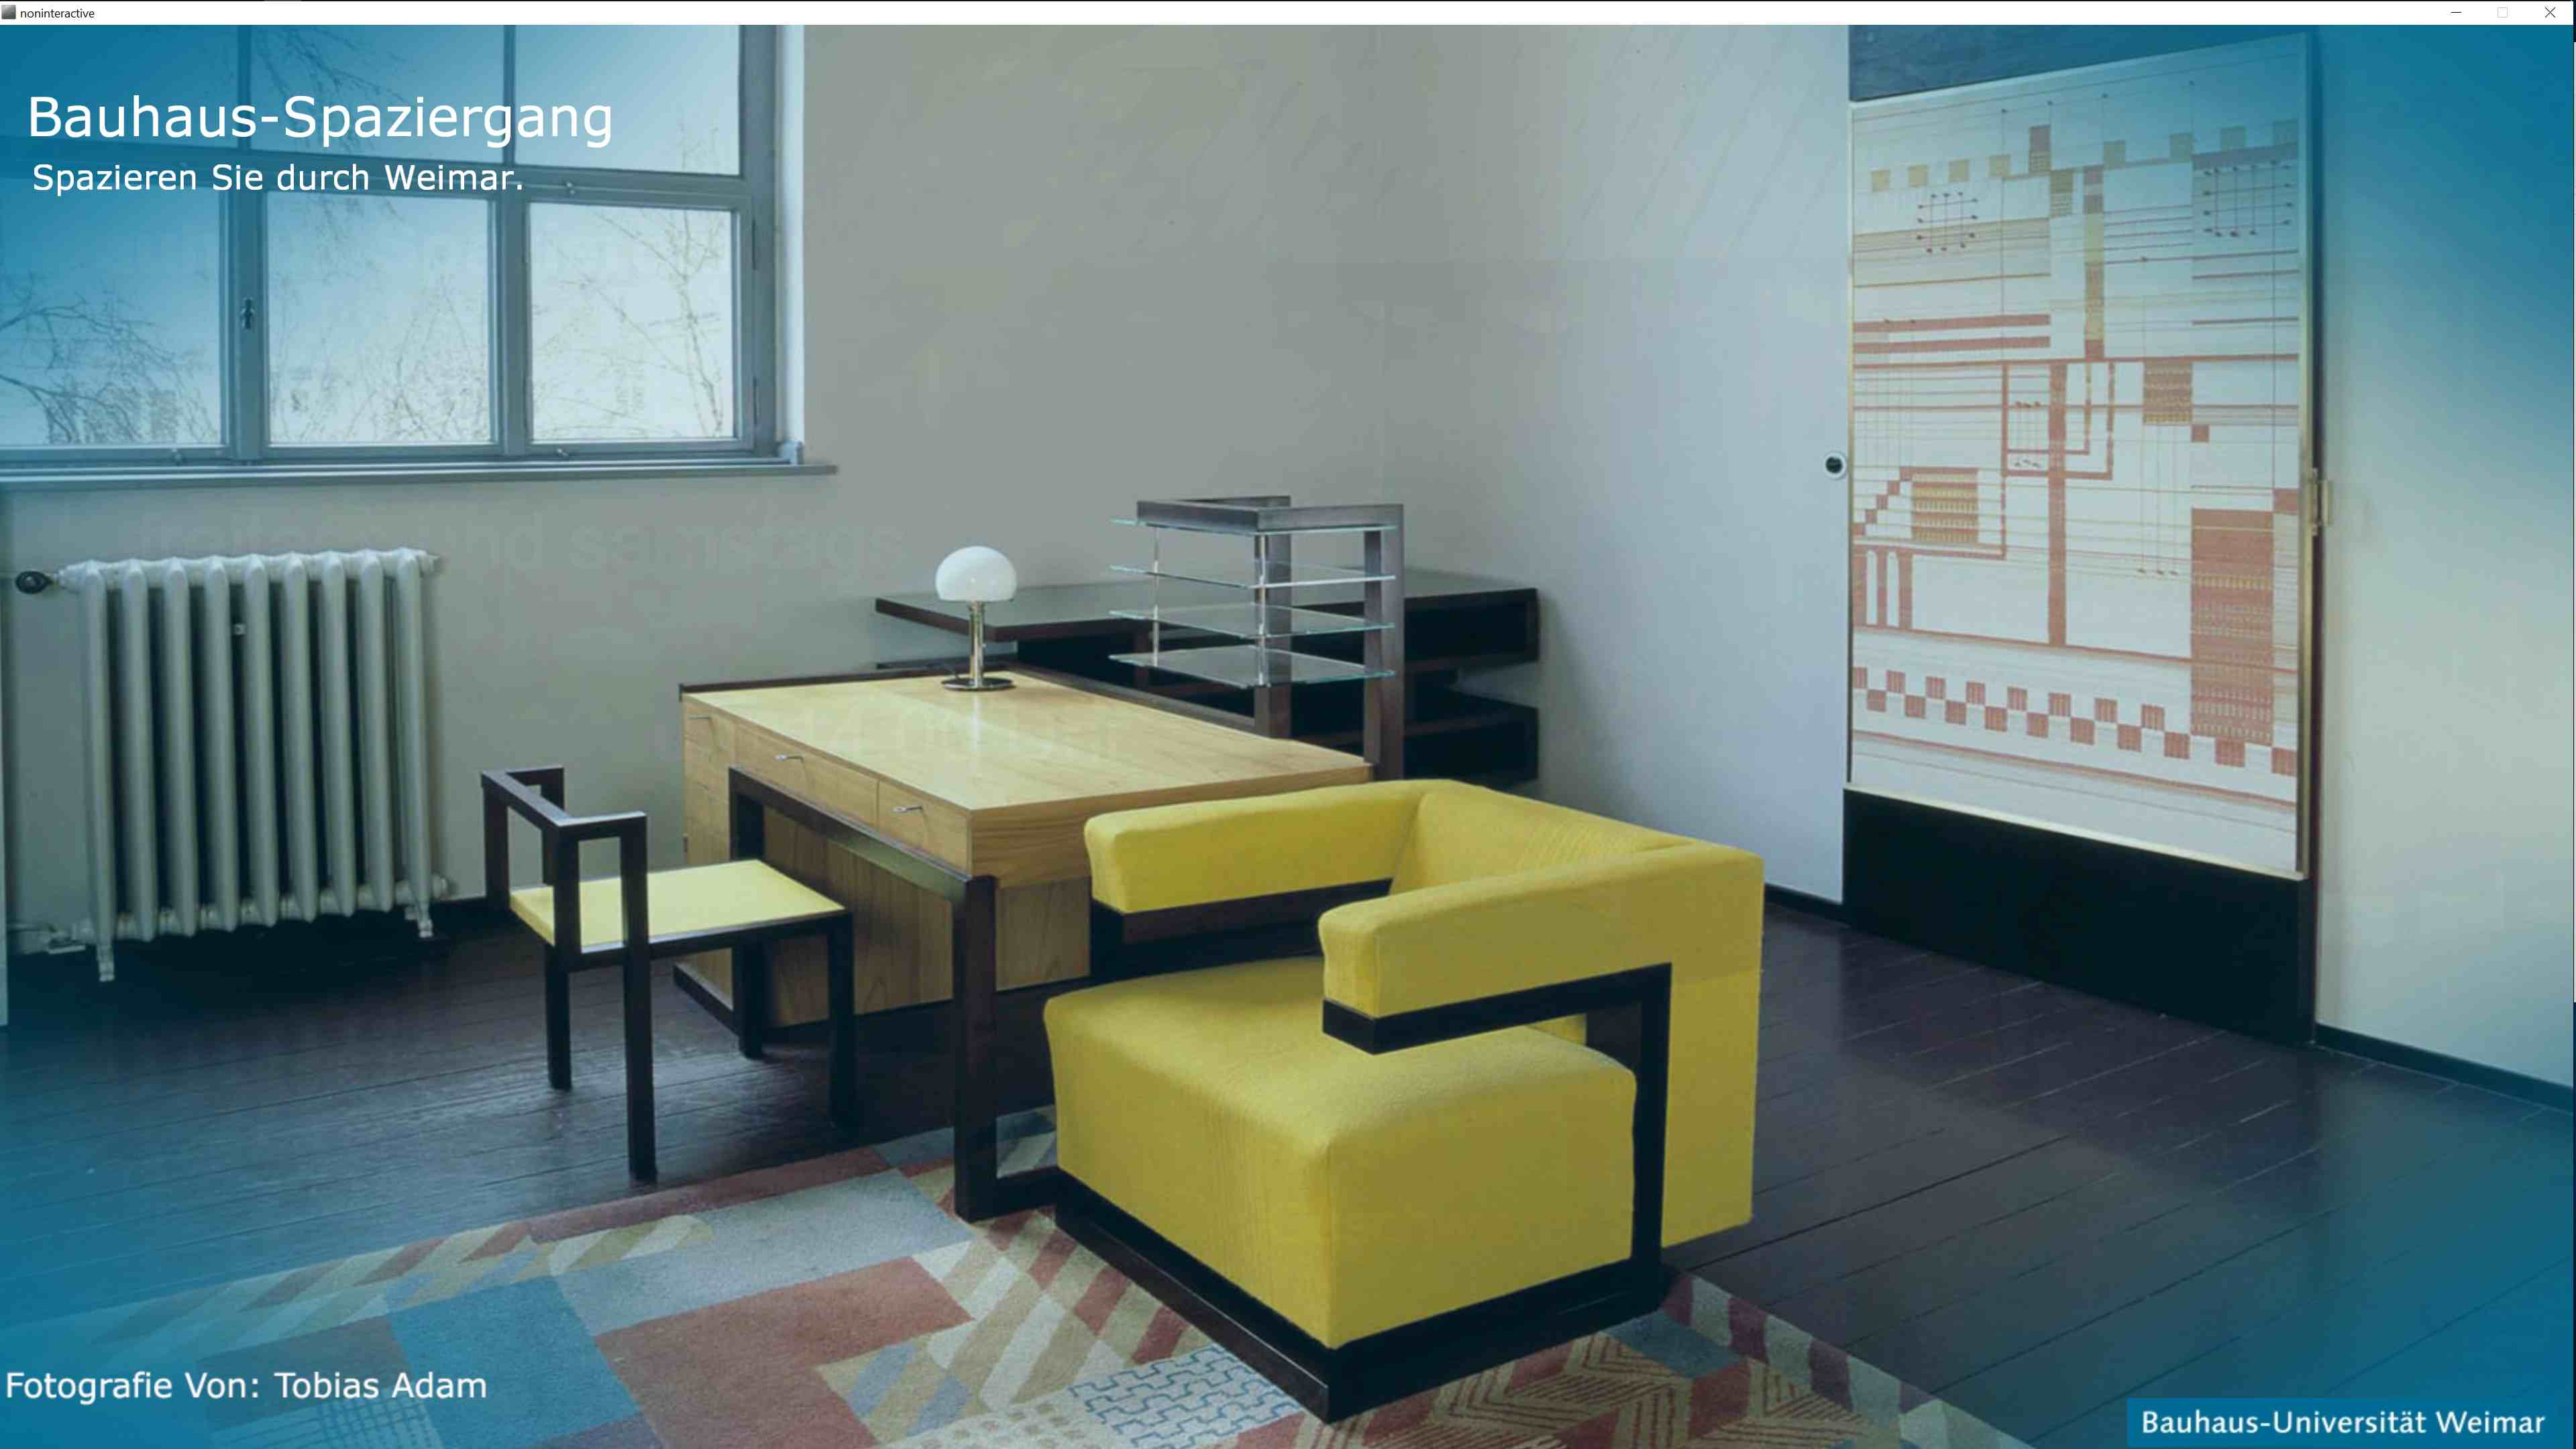
\includegraphics[width=100mm,height=60mm]{Figures/7/initialpage}
    \caption{Initial Interface}%
    \label{fig:adInitialpage}%
\end{figure}

\item Map Interface: \\
This is the city map of Weimar that has some interest regions shown on the top of the map. Those regions are blinking to signal the users.

\begin{figure}[H]
    \centering
    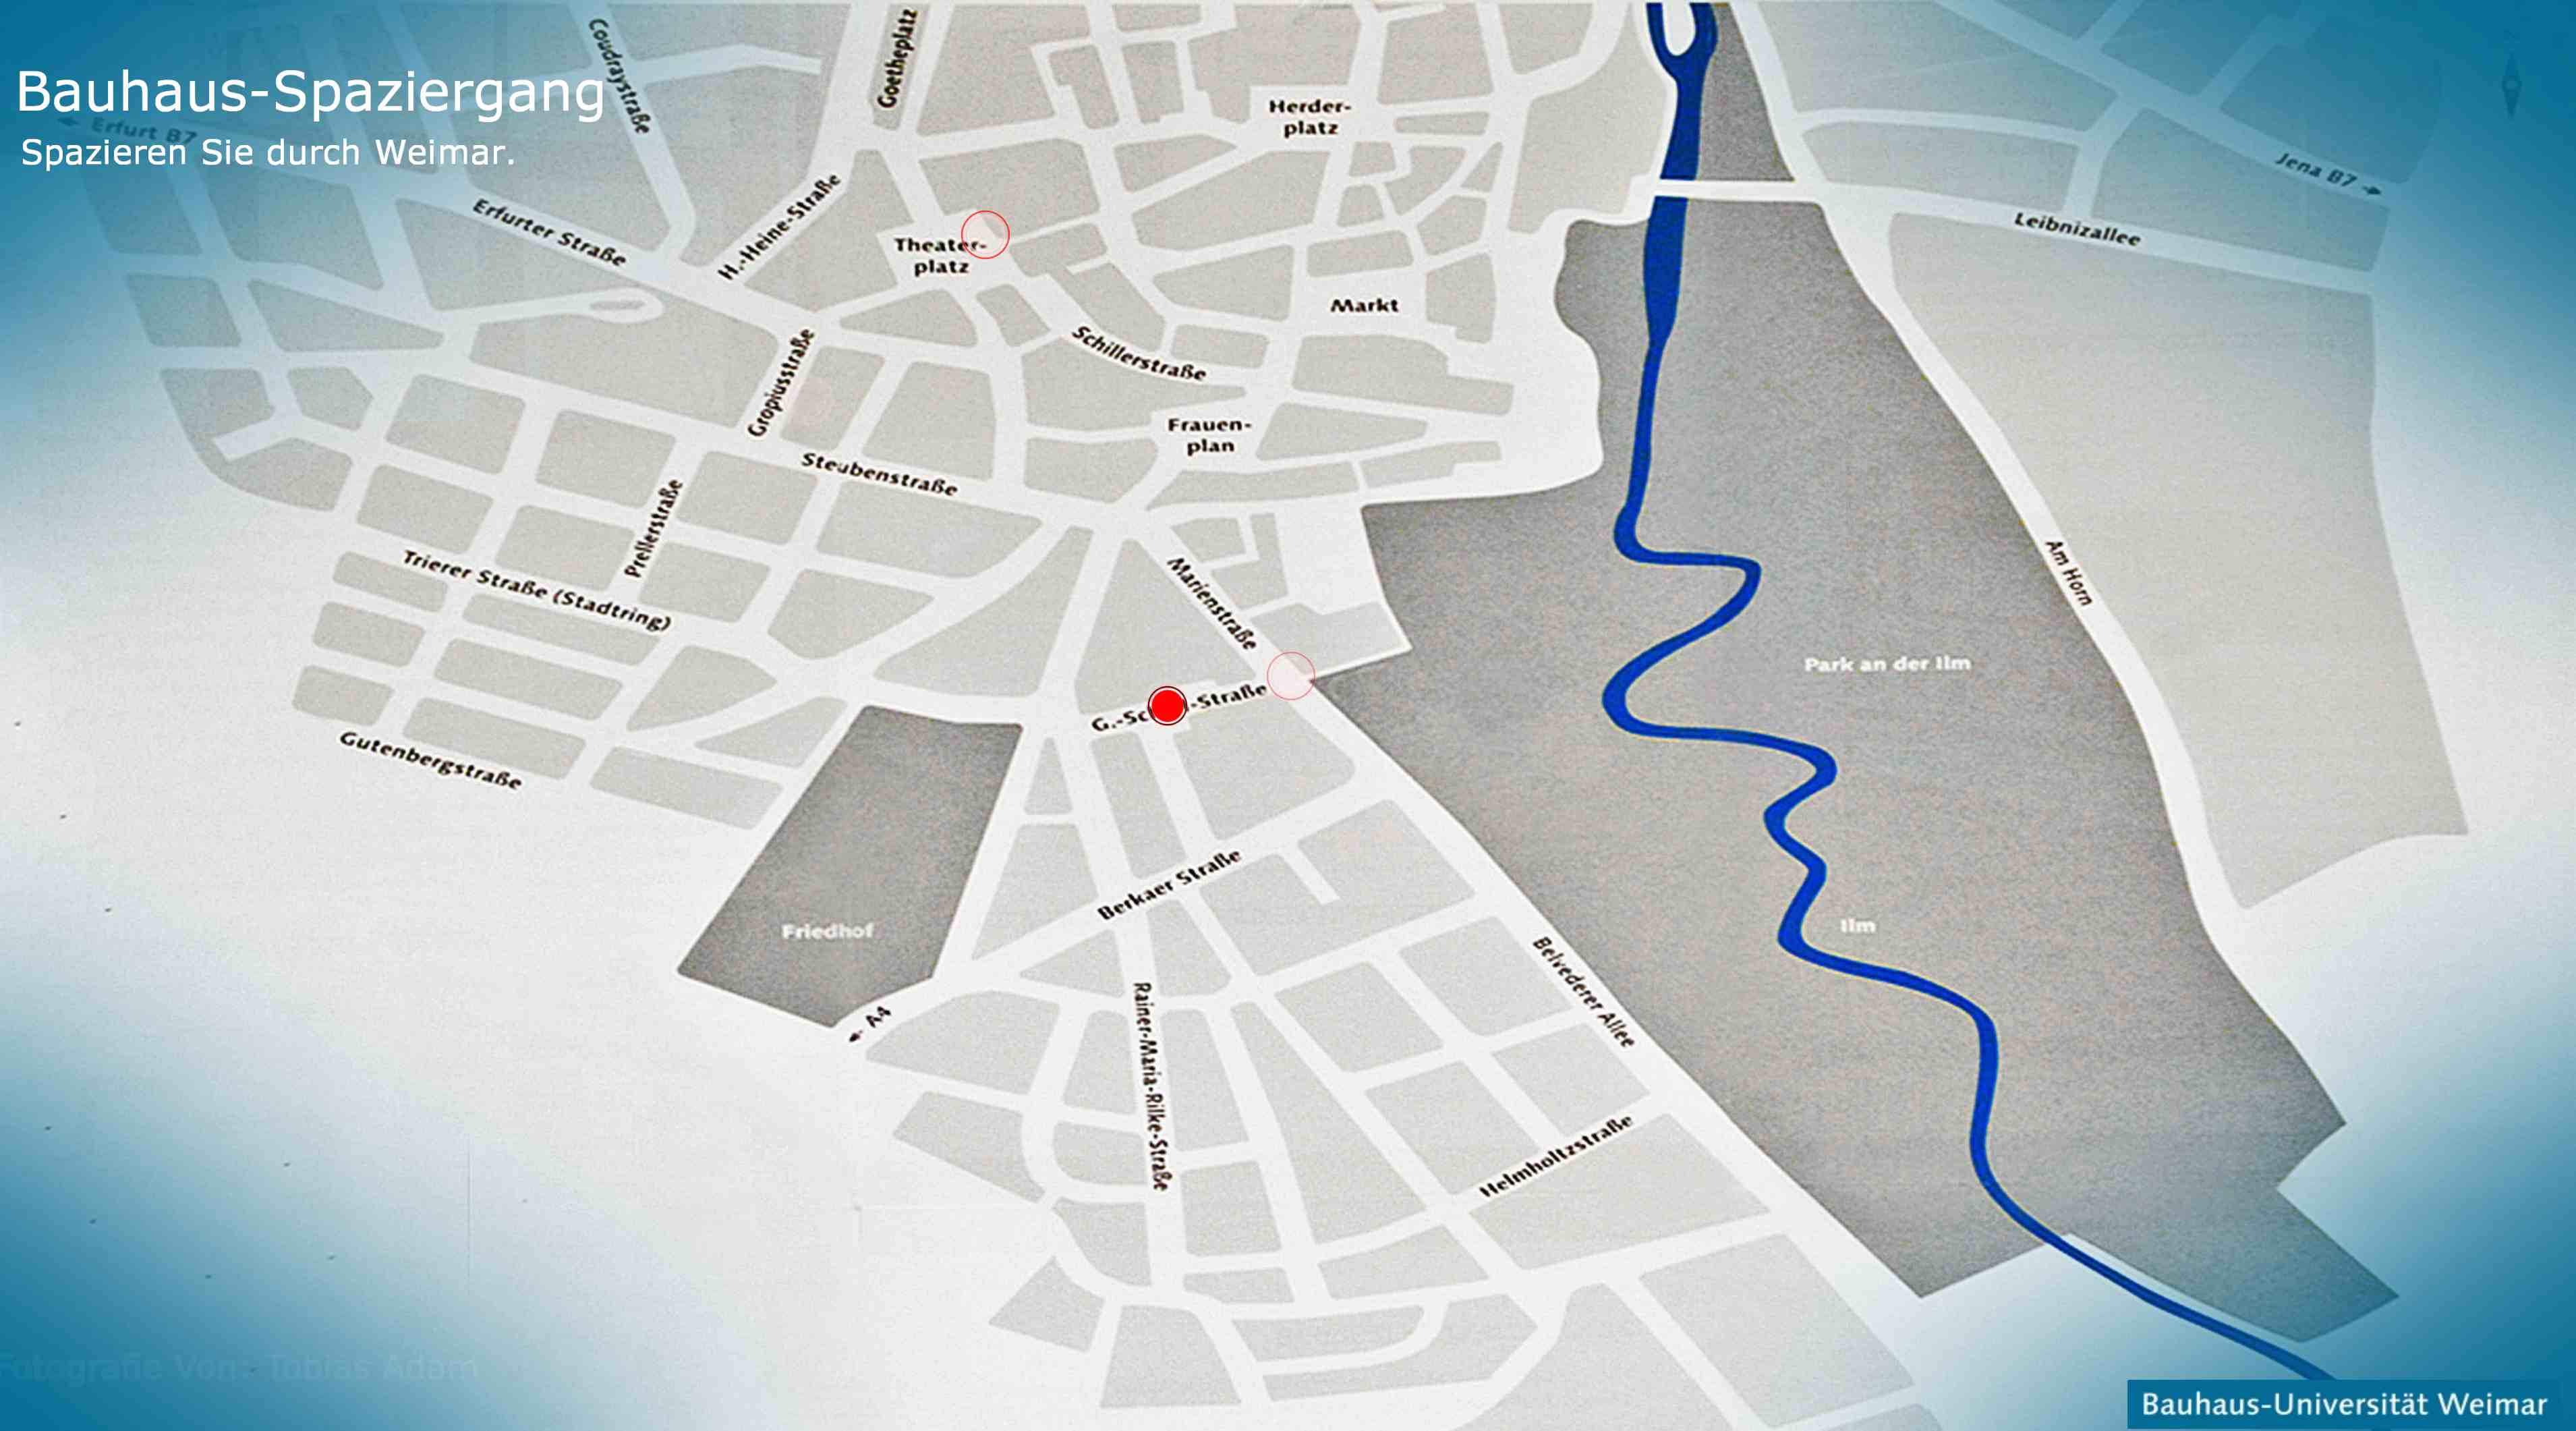
\includegraphics[width=100mm,height=60mm]{Figures/7/map}
    \caption{Map Interface}%
    \label{fig:adSecondpage1}%
\end{figure}

The location pictures are animated randomly and they are first enlarged, and then resized backed to fit on the map region.
\begin{figure}[H]
    \centering
    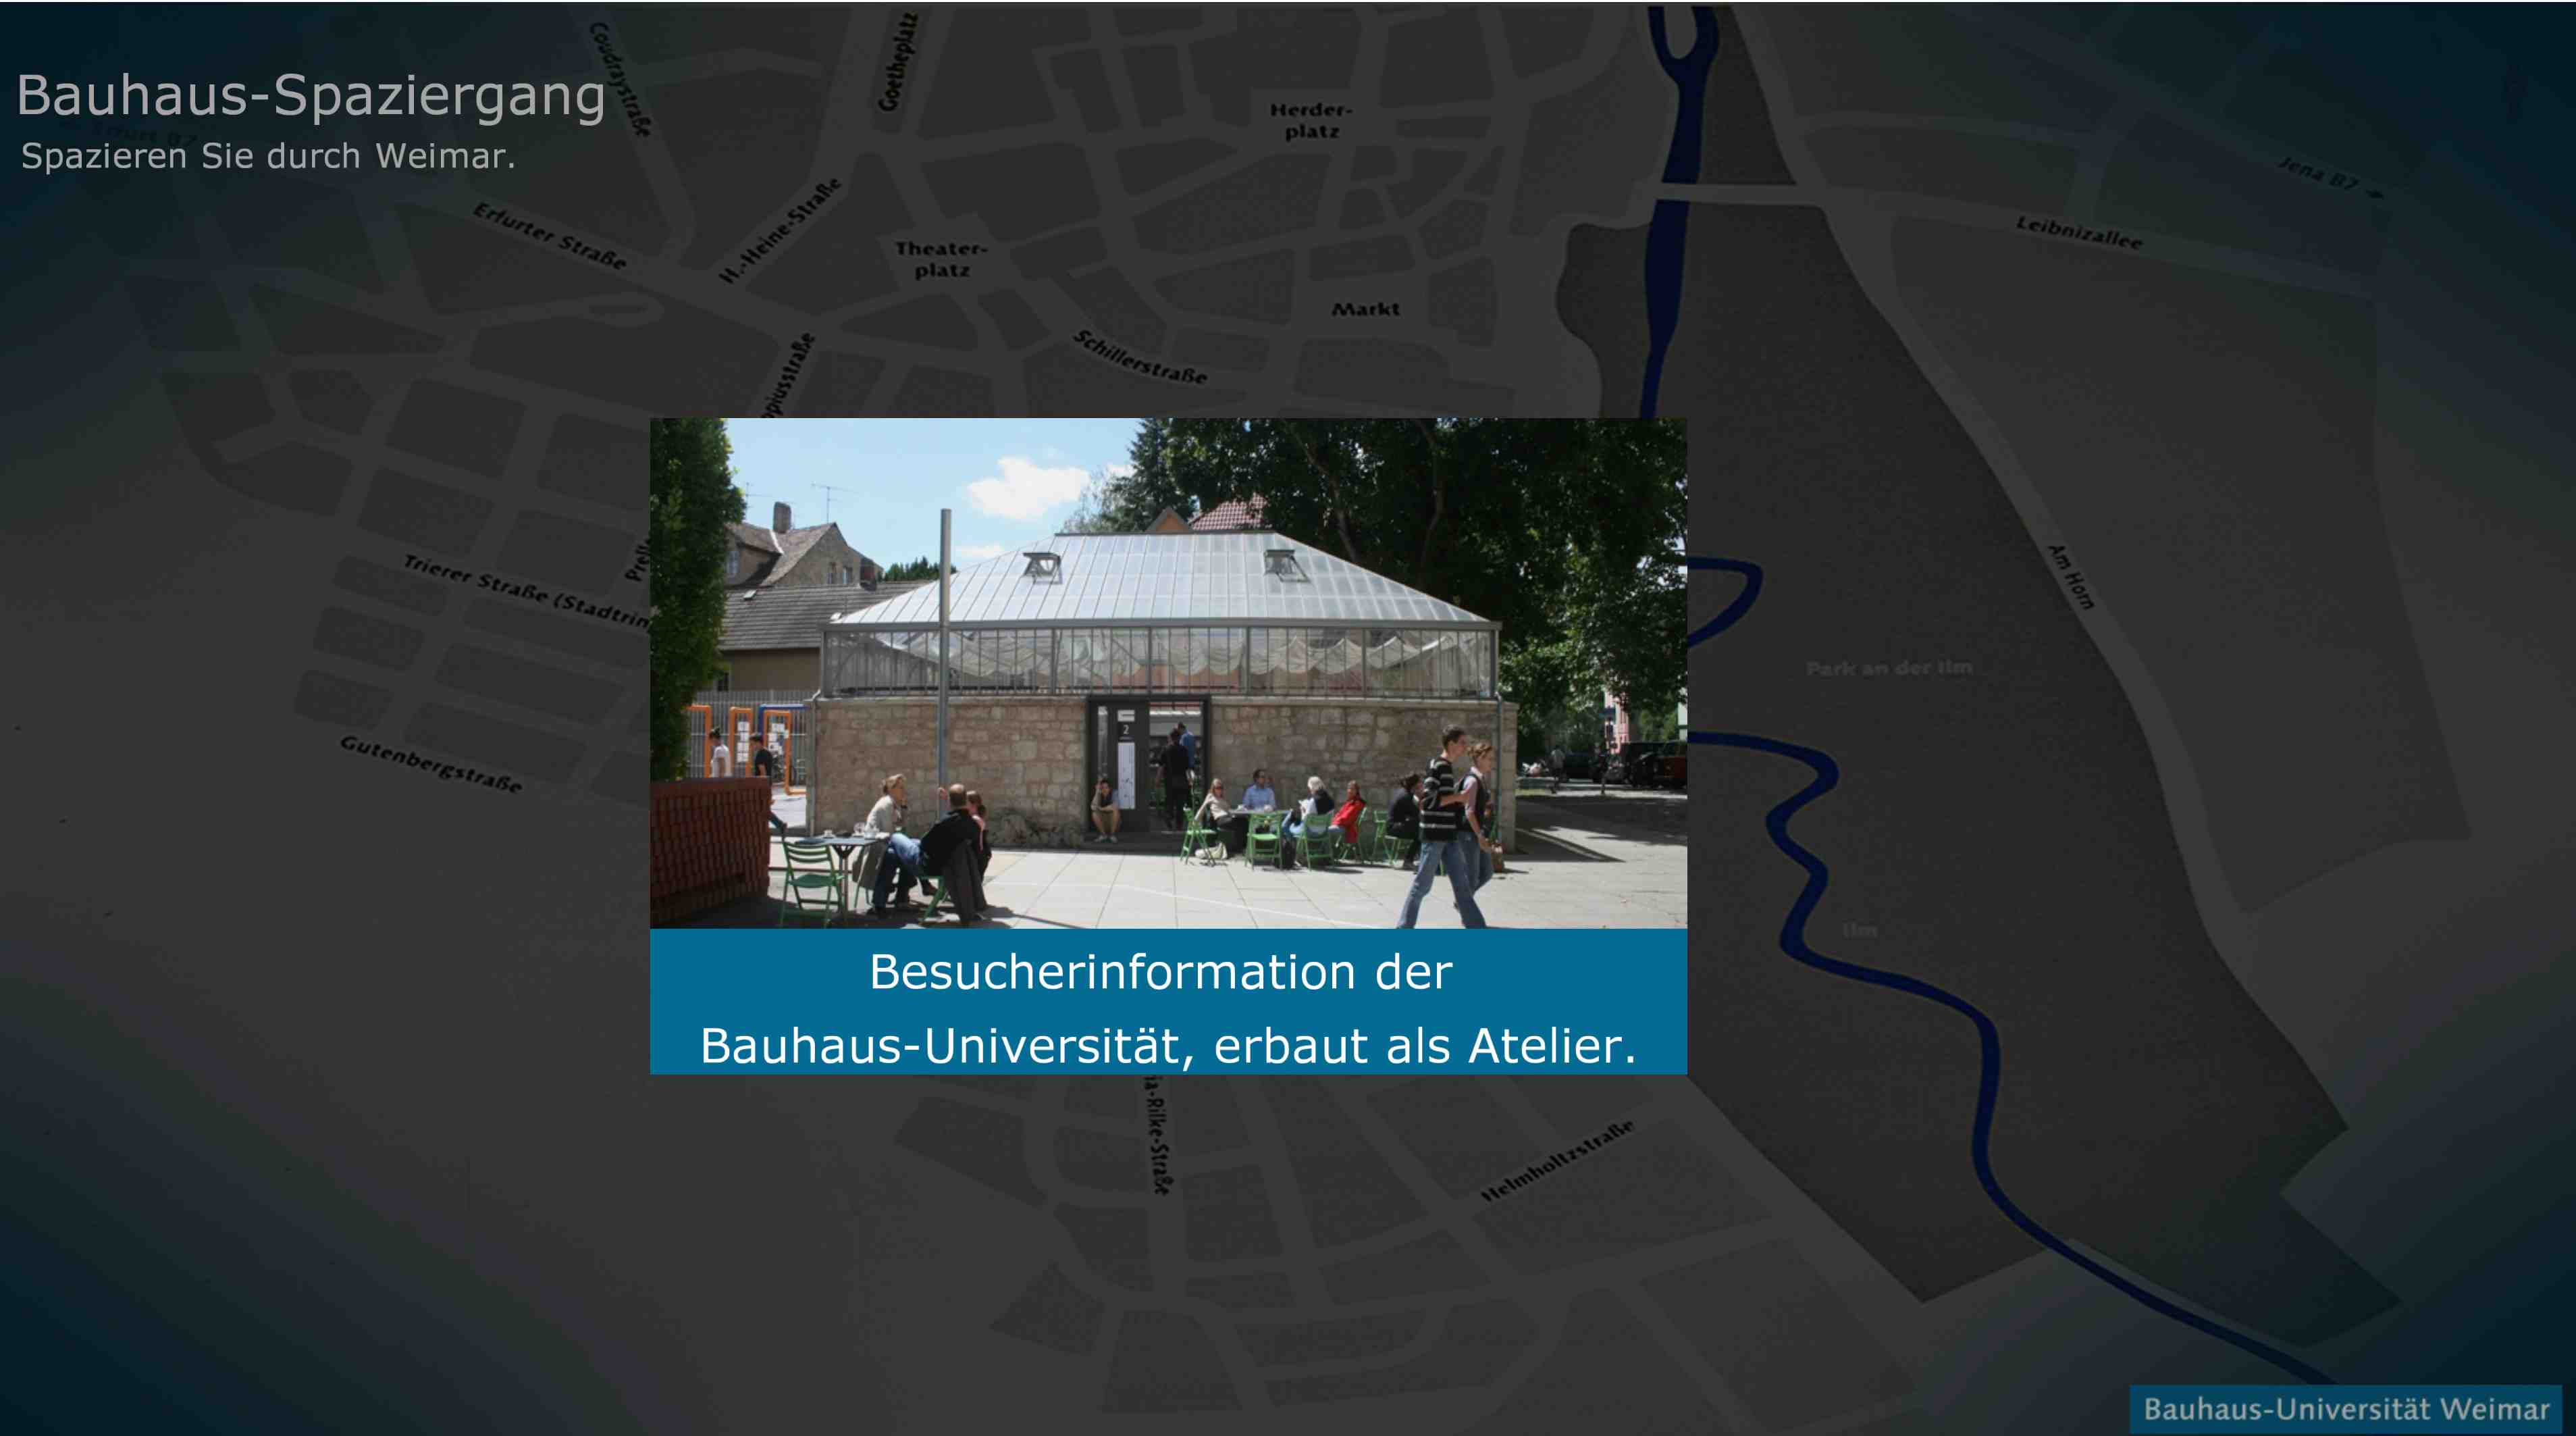
\includegraphics[width=100mm,height=60mm]{Figures/7/enlarged_pic}
    \caption{Enlarged picture}%
    \label{fig:adSecondpage2}%
\end{figure}

The resized pictures on the map looks like below. 
\begin{figure}[H]
    \centering
    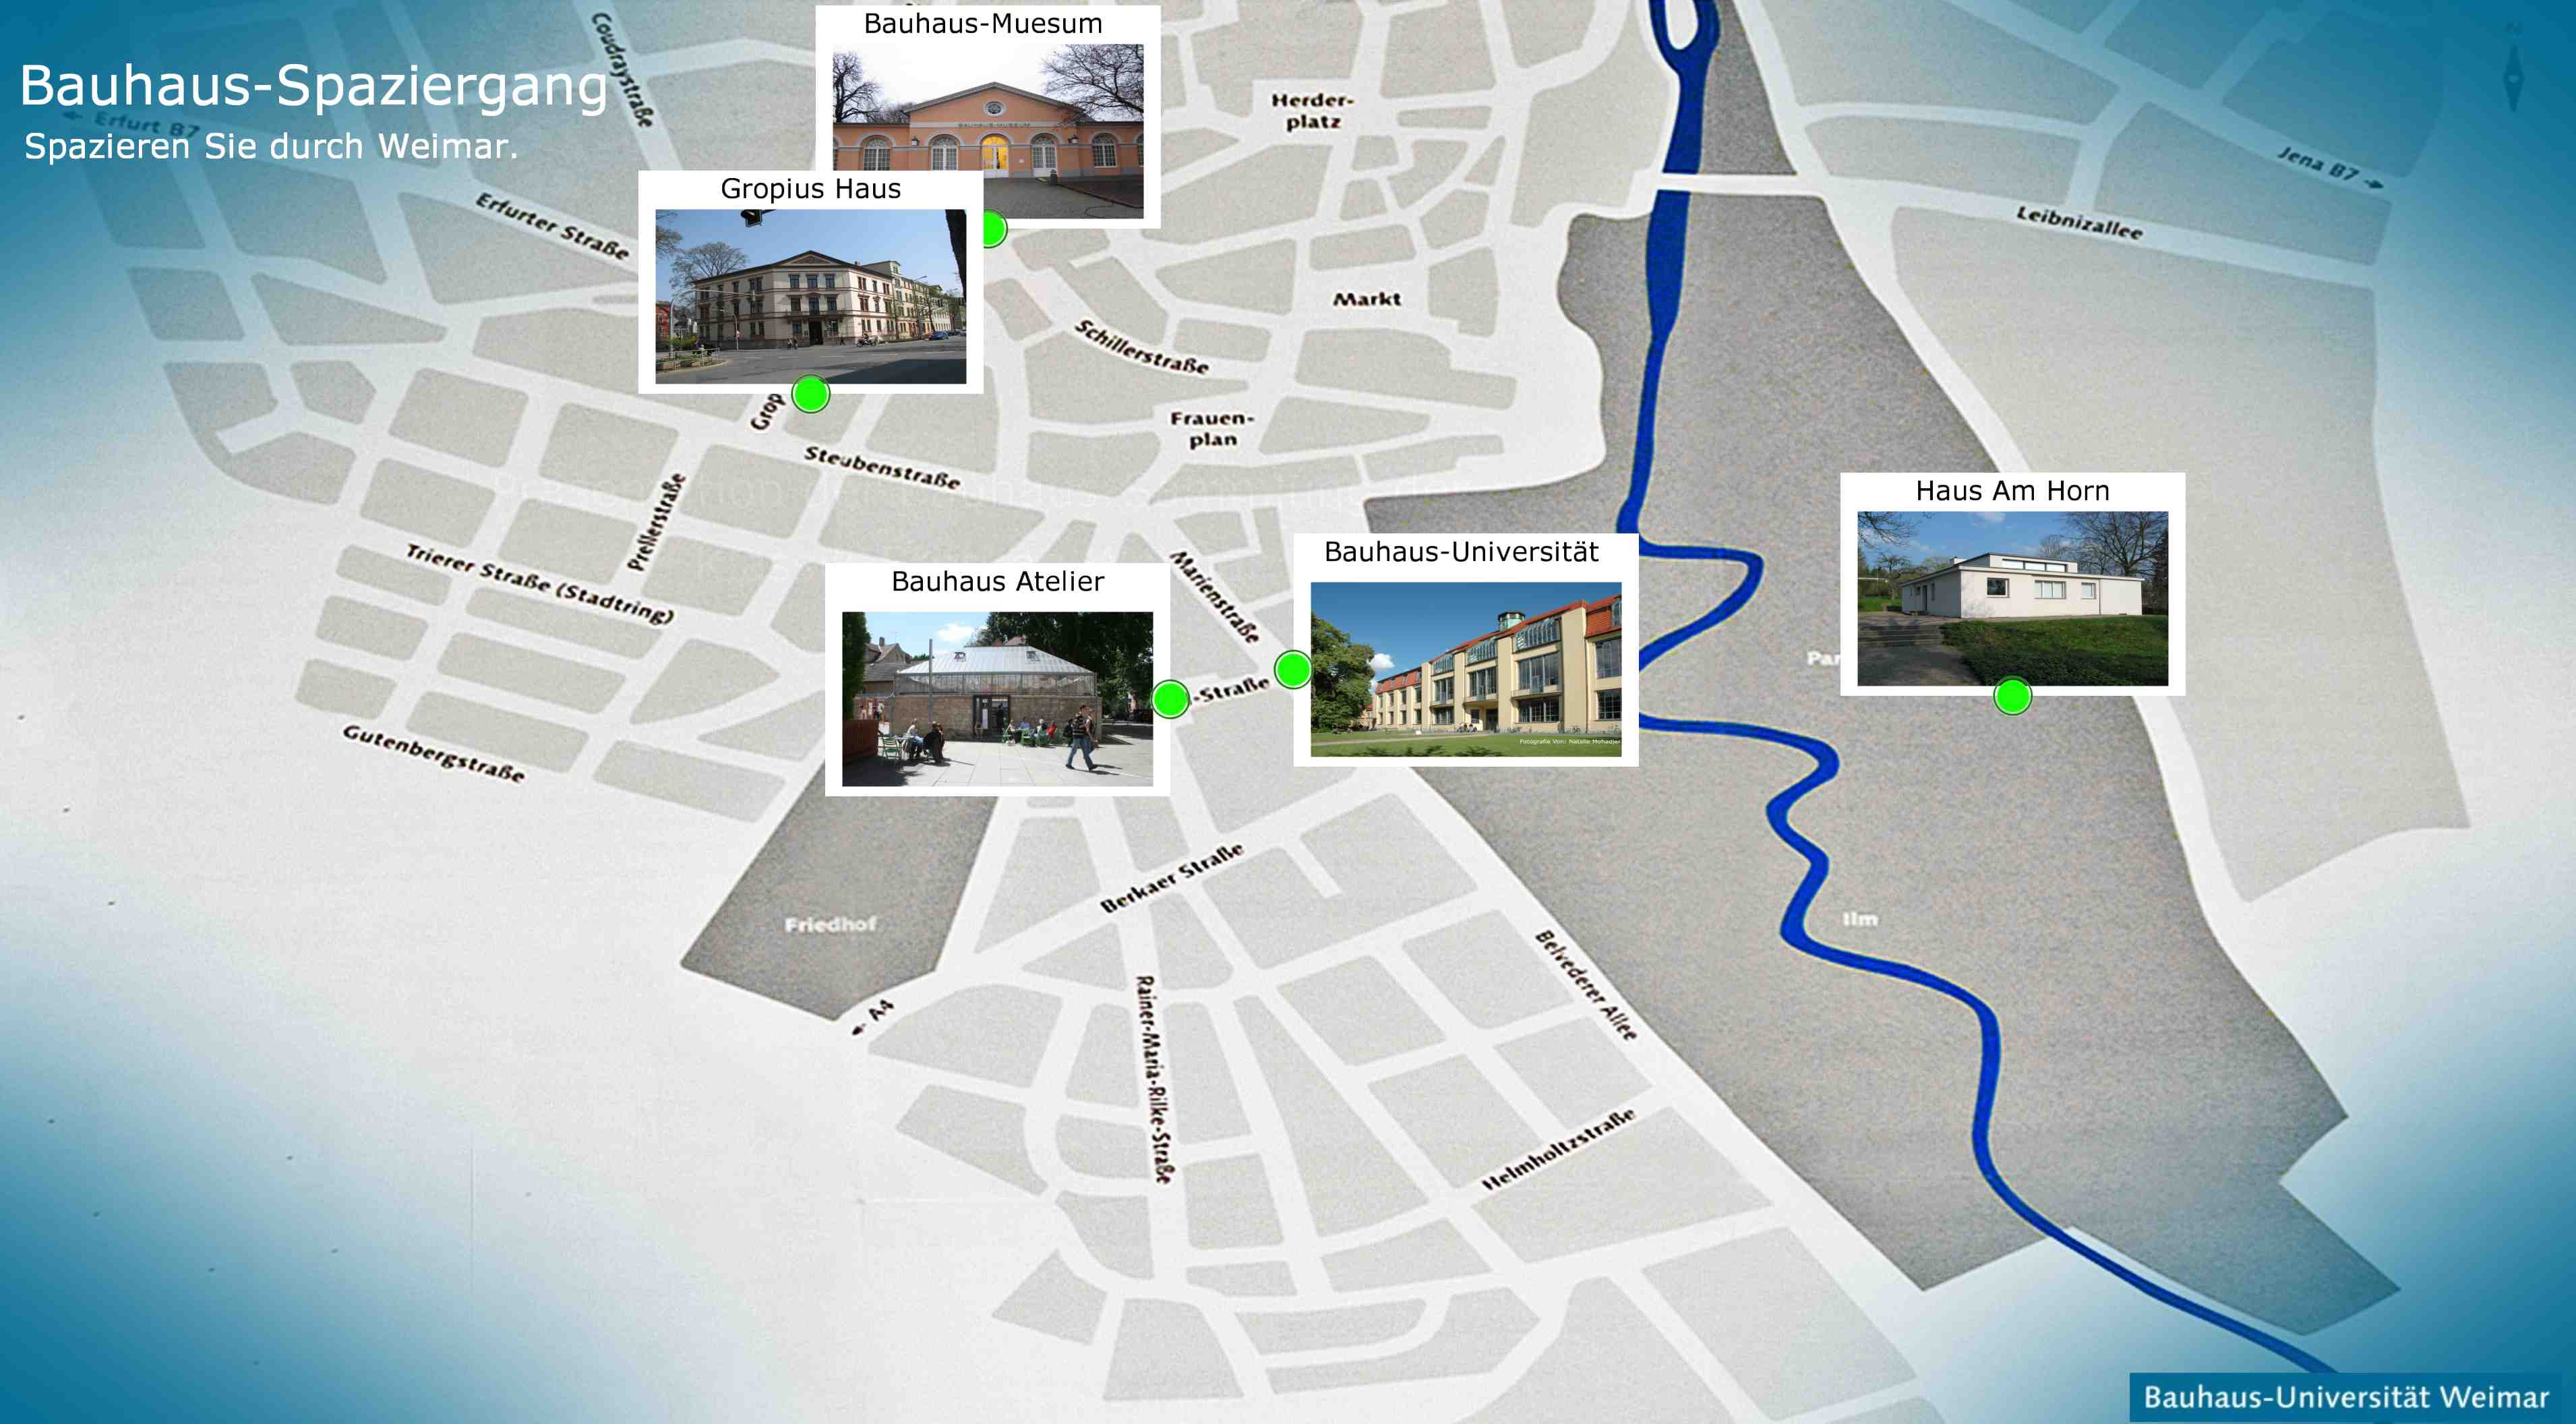
\includegraphics[width=100mm,height=60mm]{Figures/7/map_pictures}
    \caption{Pictures on the map}%
    \label{fig:adSecondpage3}%
\end{figure}

\item Advertisement video:\\
In this interface the video is being played, this picture is a screenshot of one of the frames of the video.
\begin{figure}[H]
    \centering
    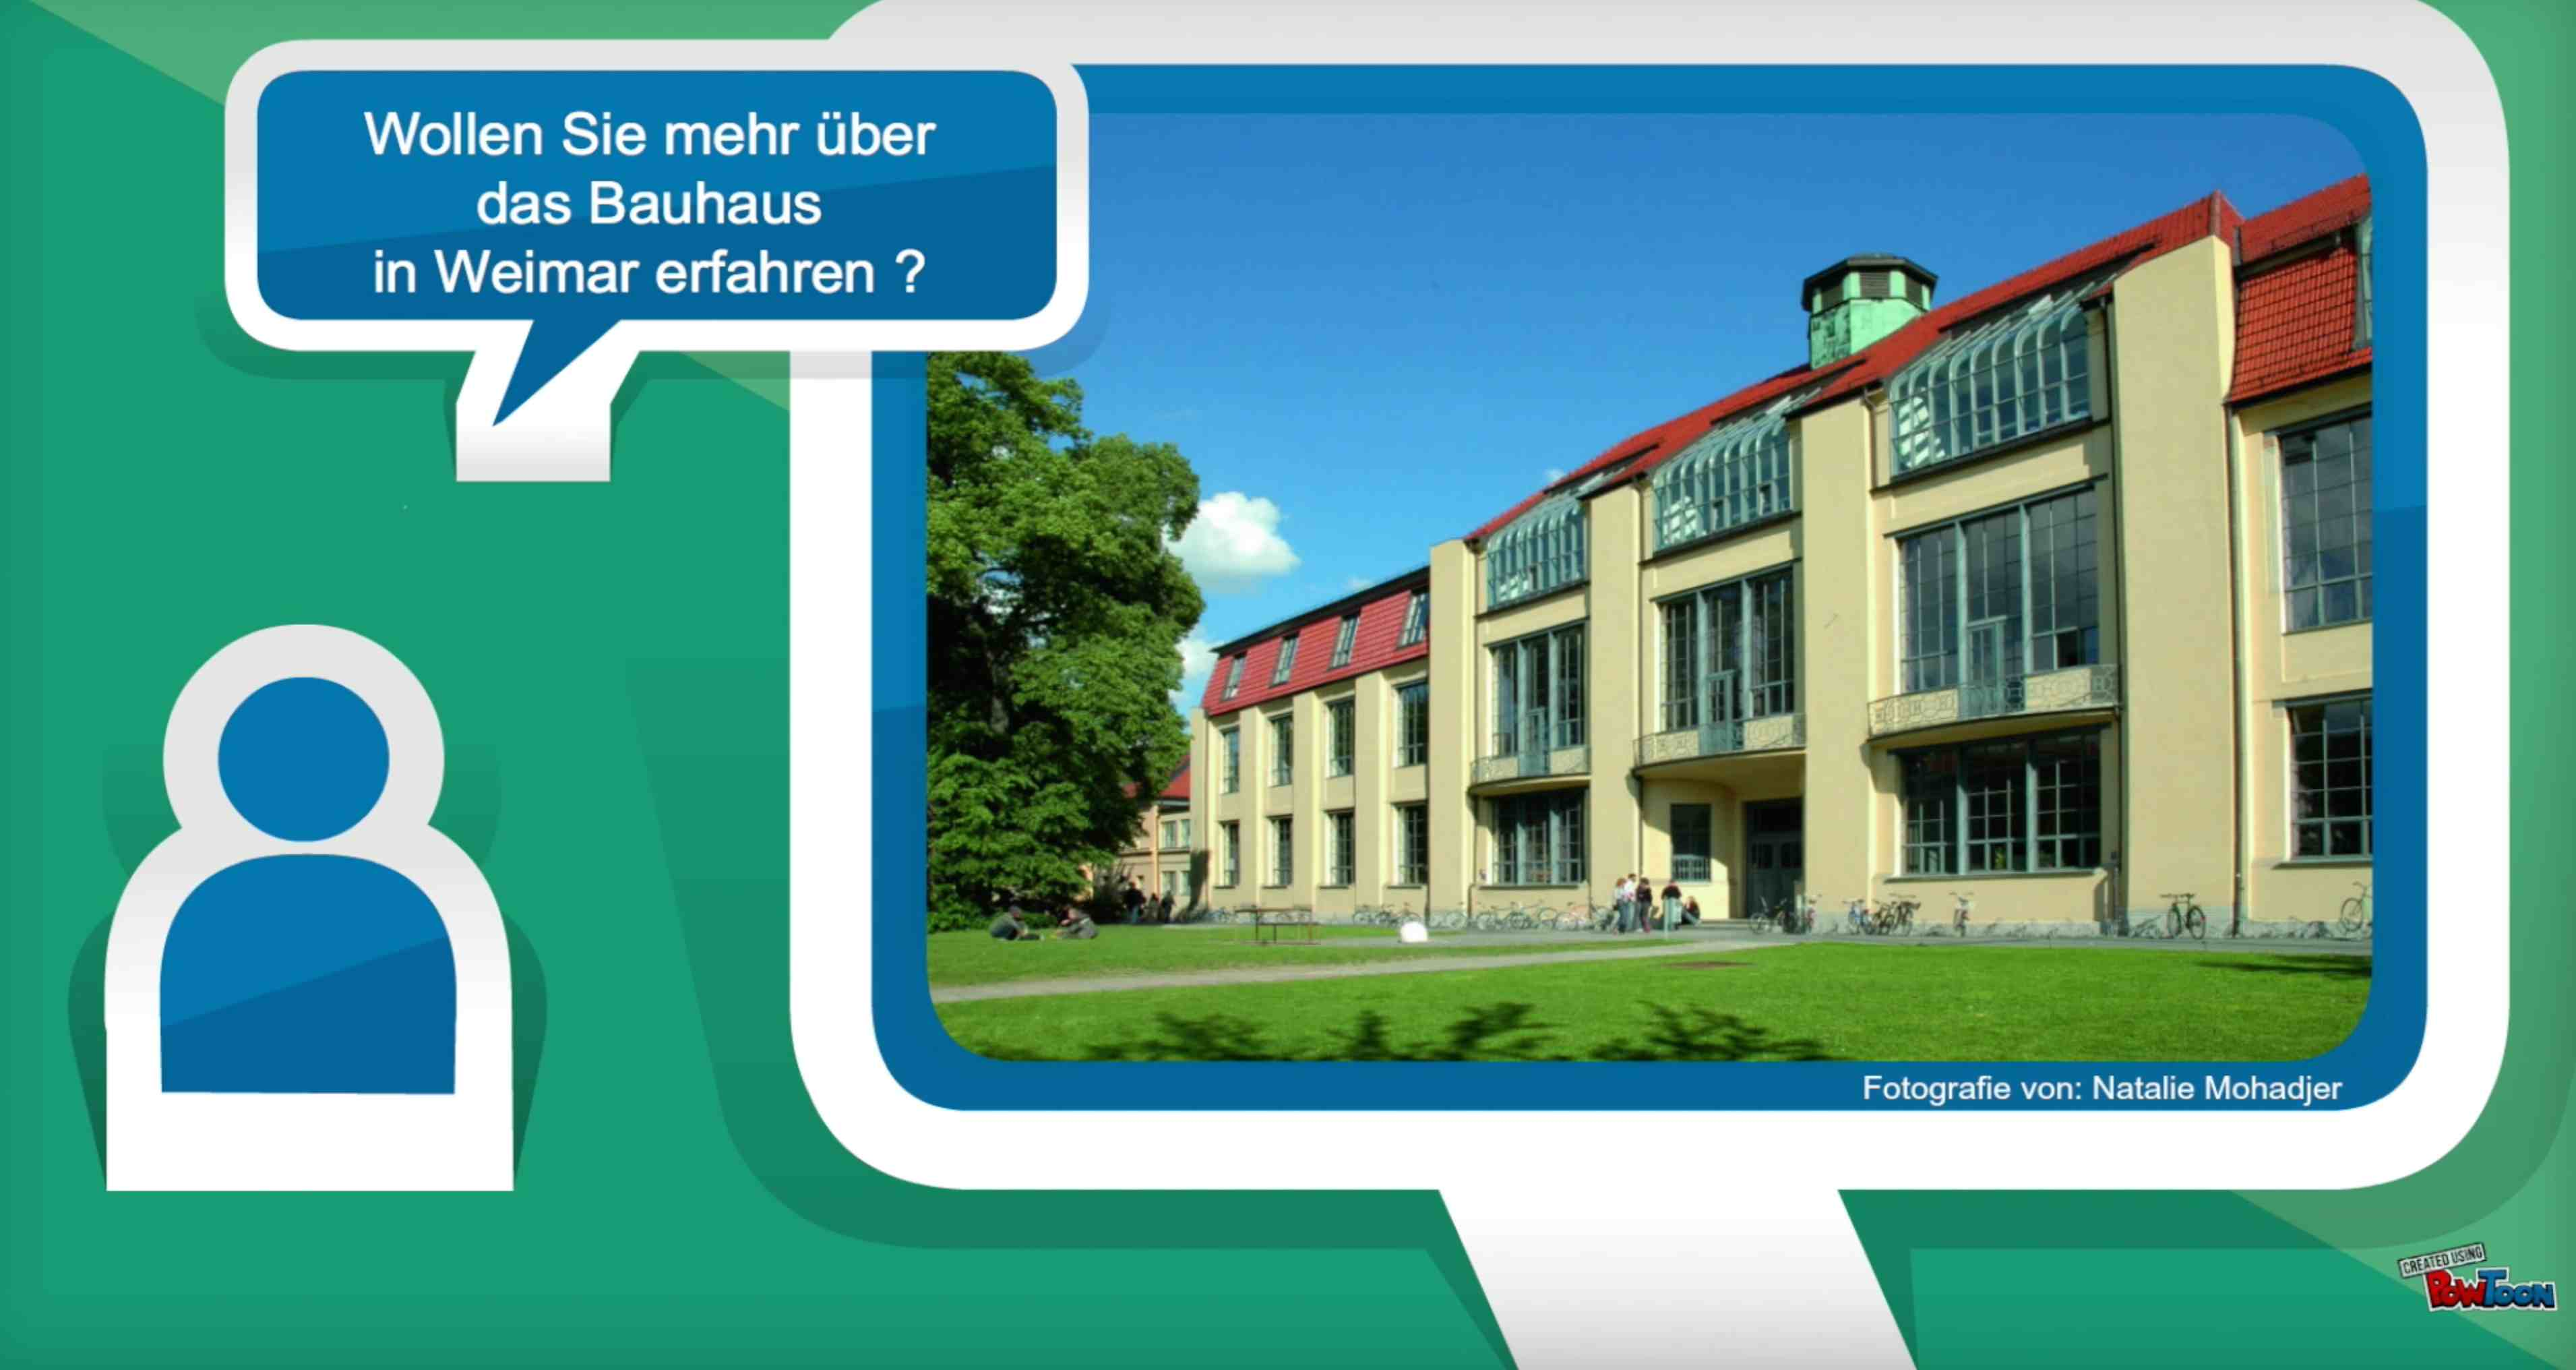
\includegraphics[width=100mm,height=60mm]{Figures/7/ad_first}
    \caption{Advertisement video}%
    \label{fig:adthirdpage1}%
\end{figure}

This is the last frame of the video that shows information about how and where to join the Bauhaus Walk.

\begin{figure}[H]
    \centering
    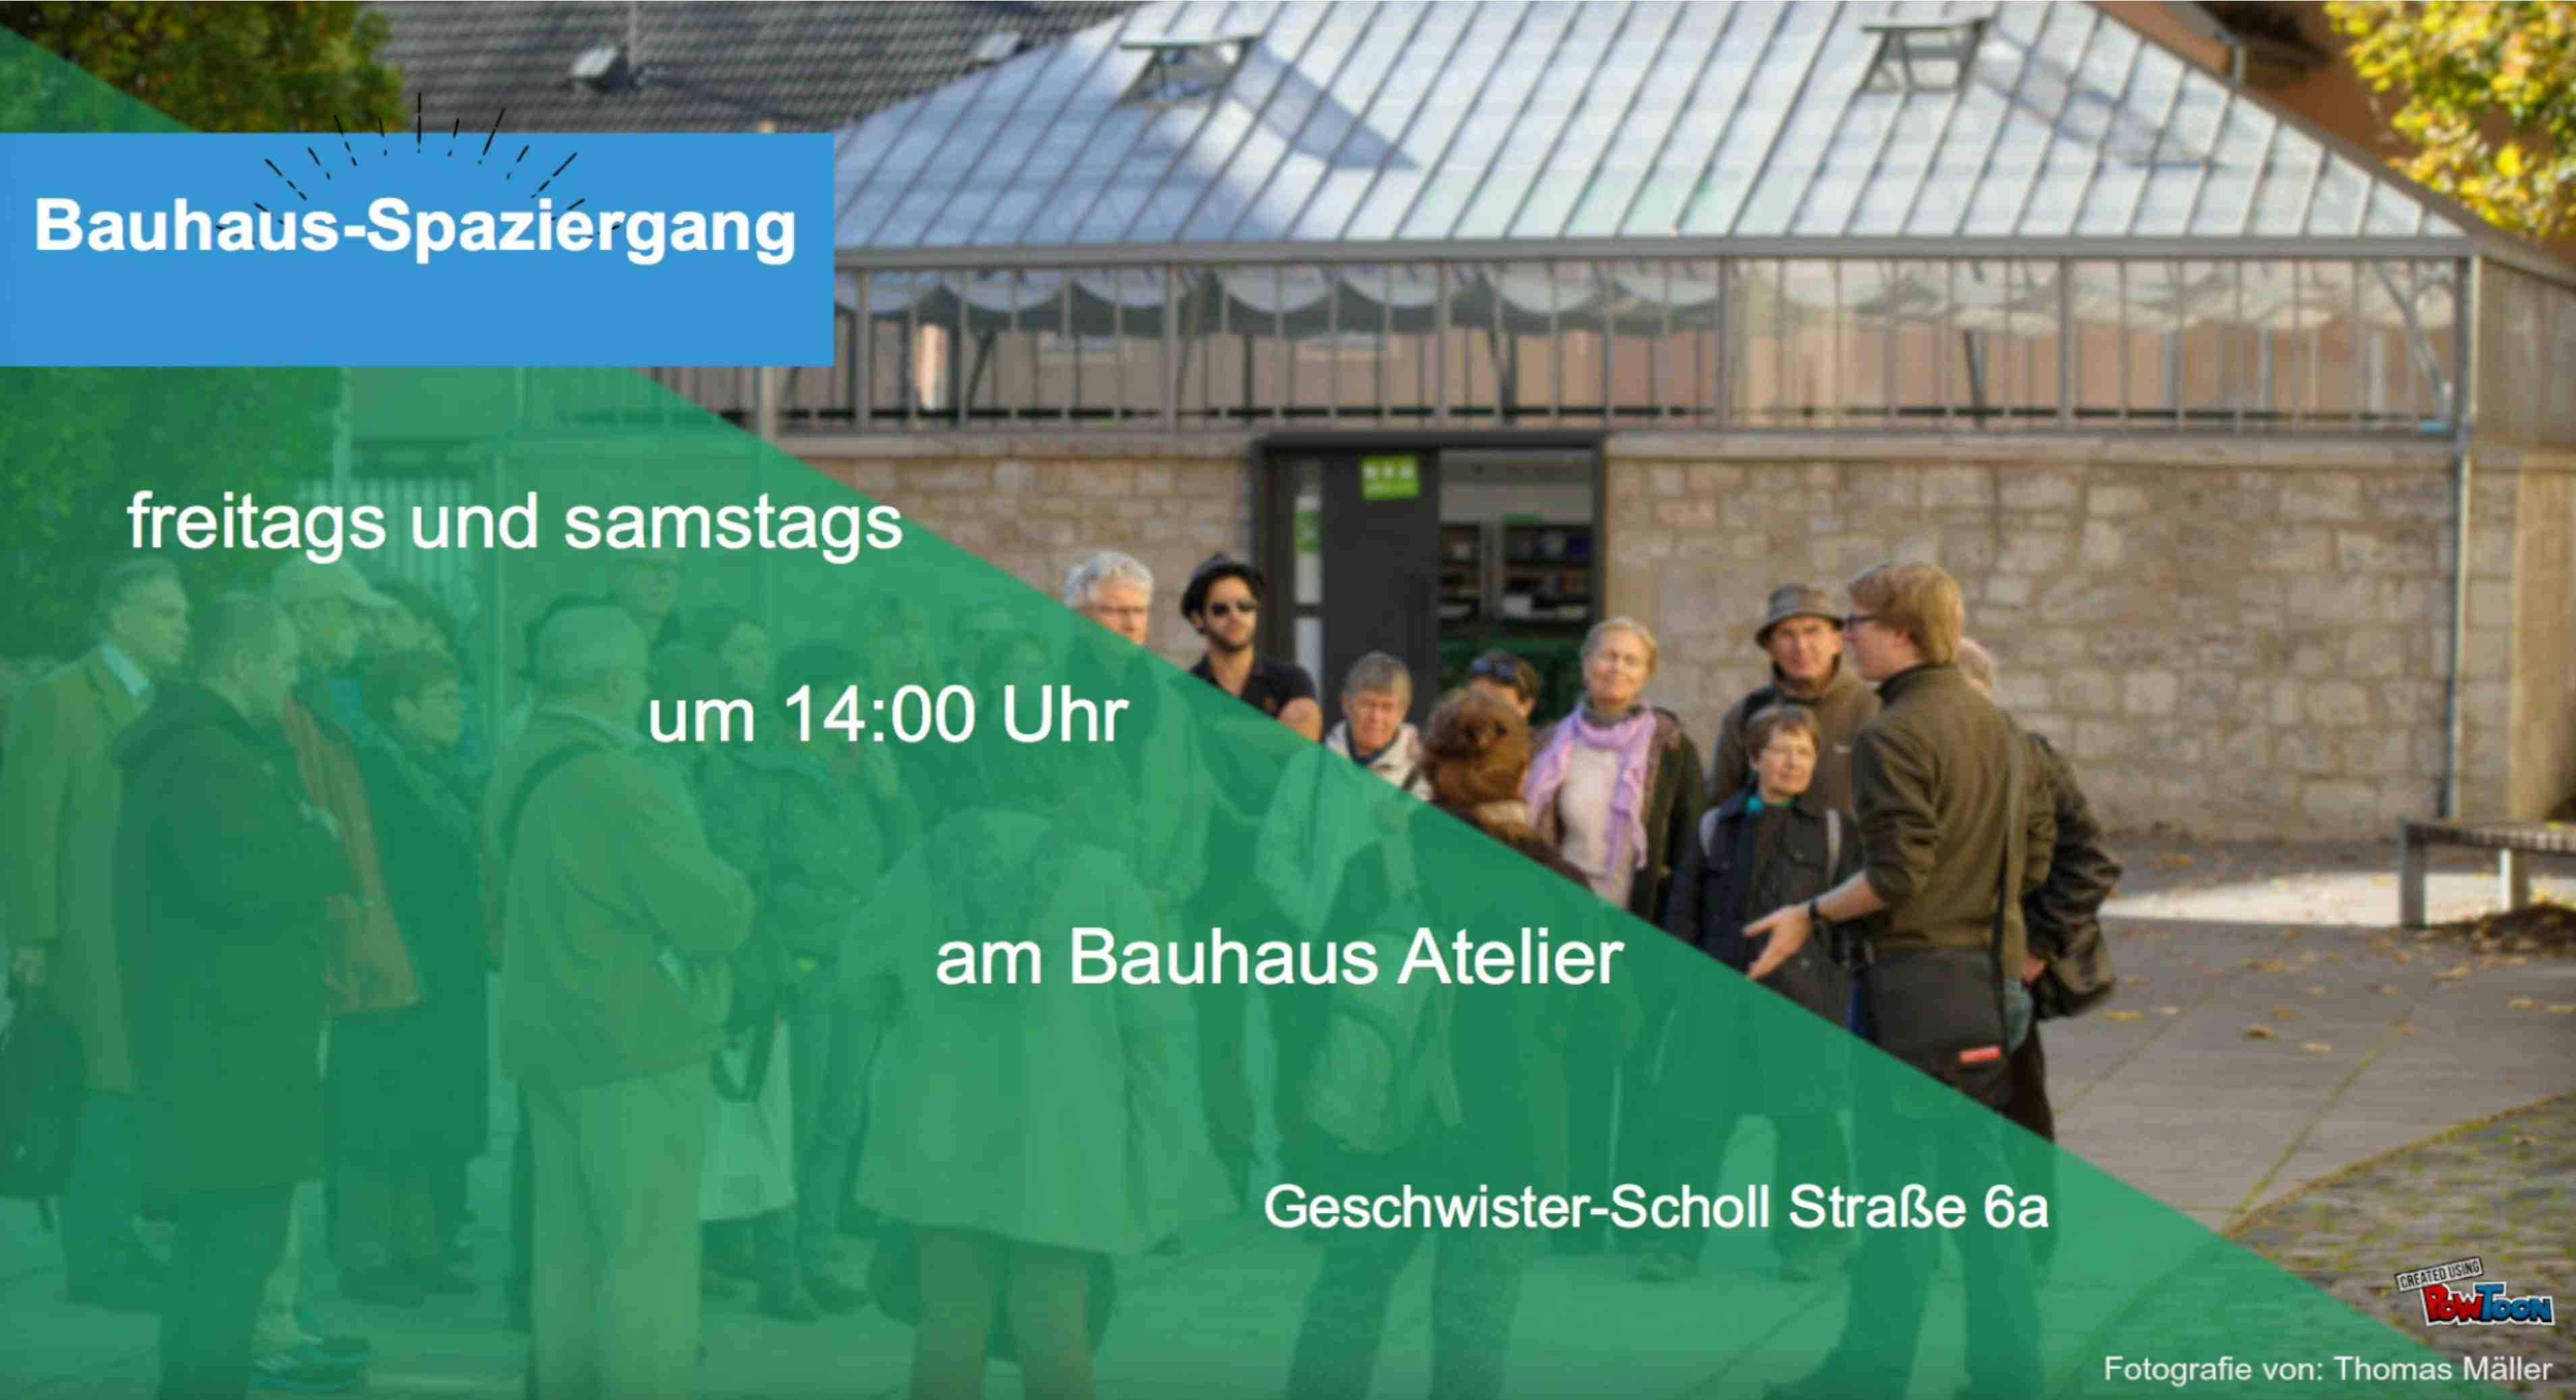
\includegraphics[width=100mm,height=60mm]{Figures/7/ad_last}
    \caption{Advertisement video last frame}%
    \label{fig:adthirdpage2}%
\end{figure}

The advertisement video was created in PowToon\footnote{PowToon: \url{https://www.powtoon.com/index/?gclid=CJqSqrf5l80CFesV0wod1u8IEQ&edgetrackerid=10083804111572}, last accessed 5 jun 2016} with a free version account, visit this video\footnote{Advertisement Video:  \url{https://www.youtube.com/watch?v=-y1Dbz6E6bU&feature=youtu.be}, last accessed 5 jun 2016} that shows the advertisement video or browse the animation from the DVD. 

To see the full the non-interactive advertisement flow of the interfaces and its animations visit this video\footnote{Non-interactive Ad: \url{https://www.youtube.com/watch?v=ZLszzfbZJgI}, last accessed: 5 Jun 2016} or browse the video from DVD.


\end{enumerate}

\iffalse
\subsection{Hardware setup}
The below setup is the hardware setup for the advertisement. The same setup is used for all three weeks.

\begin{figure}[H]
    \centering
    \includegraphics[width=100mm,height=70mm]{Figures/7/Physical_setup}
    \caption{Hardware setup}%
    \label{fig:hardwaresetup}%
\end{figure}


\hilight{put the picture of the screen here}

\begin{figure}[H]
    \centering
    \includegraphics[width=100mm,height=70mm]{Figures/7/Physical_setup}
    \caption{Picture}%
    \label{fig:hardwaresetup}%
\end{figure}



\subsubsection{Flowchart Diagram}

\begin{figure}[H]
    \centering
    \includegraphics[width=100mm,height=90mm]{Figures/7/Non-interactive/flow_chart_diagram}
    \caption{Non-interactive Flowchart diagram}%
    \label{fig:non_inter_flowchart}%
\end{figure}
\fi


\subsubsection{Body Interactive application}
As discussed earlier, there are three interfaces or phases (initial interface, map interface and advertisement video) of the application, and in body interaction the same interfaces are used, but two of them are interactive. The first two interfaces are interactive and allow participants to interact with using their body like exploring the interest points on the map by moving physically (forward, backward, right and left) in front of the screen. The last interface shows advertisement video, which is not interactive.  All the interfaces are explained in the following sections.

\begin{enumerate}

\item Initial Interface (\emph{Call-to-Action}) : \\
This interface is basically the same interface as the non-interactive but with a difference. It projects passersby silhouette on the interface, this interface is also called \emph{Call-to-Action} interface because it calls passers-by to interact with the screen. As can be seen in the below picture, there is someone standing in front of the screen and the interface calls him to come near. This interface also has alert messages on the top right corner of screen that alerts the participant if they move away from the camera range. In this example a second person had got untracked from the camera and the system has shown that message to raise his hand to be tracked again.

\begin{figure}[H]
    \centering
    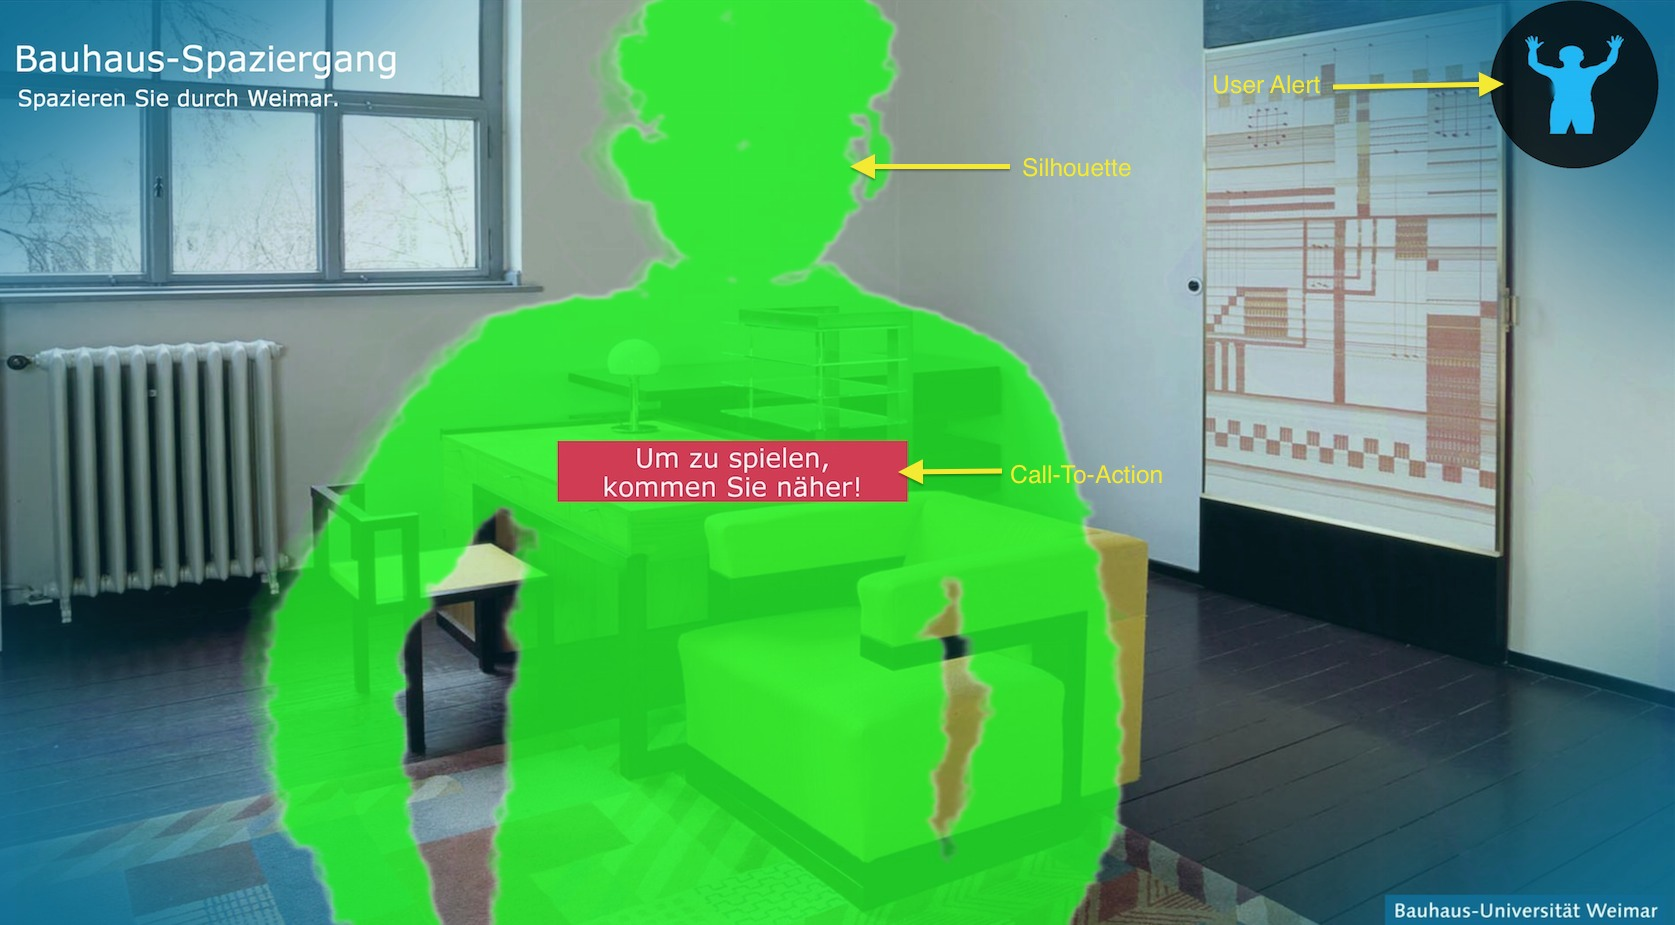
\includegraphics[width=0.8\textwidth,height=70mm]{Figures/7/body_interactive/first_interface}
    \caption{Initial interface}%
    \label{fig:body_firstinterface}%
\end{figure}


\item Transition to Map Interfaces: \\
The transition happens when the person stands close to the screen for more than 3 seconds and the processes is as follow.

\begin{enumerate}
\item Loading animation:\\
 The loading animation is a reaction to the action of the participants, which gives the user a clue that the interaction will be started. 
\item Scaling down the silhouette: \\
To walk freely on the map environment and to give the participant the feeling of real walking. The participant's silhouette is scaled down, the scaling happens smoothly frame-by-frame.
\item Show task instruction:  \\
Every interaction has instructions, the instruction is fairly very easy and it is simplified in one sentence to explore locations on the map.
\end{enumerate}

\begin{figure}[H]
    \centering
    \begin{subfigure}[H]{0.32\textwidth}
        \centering
        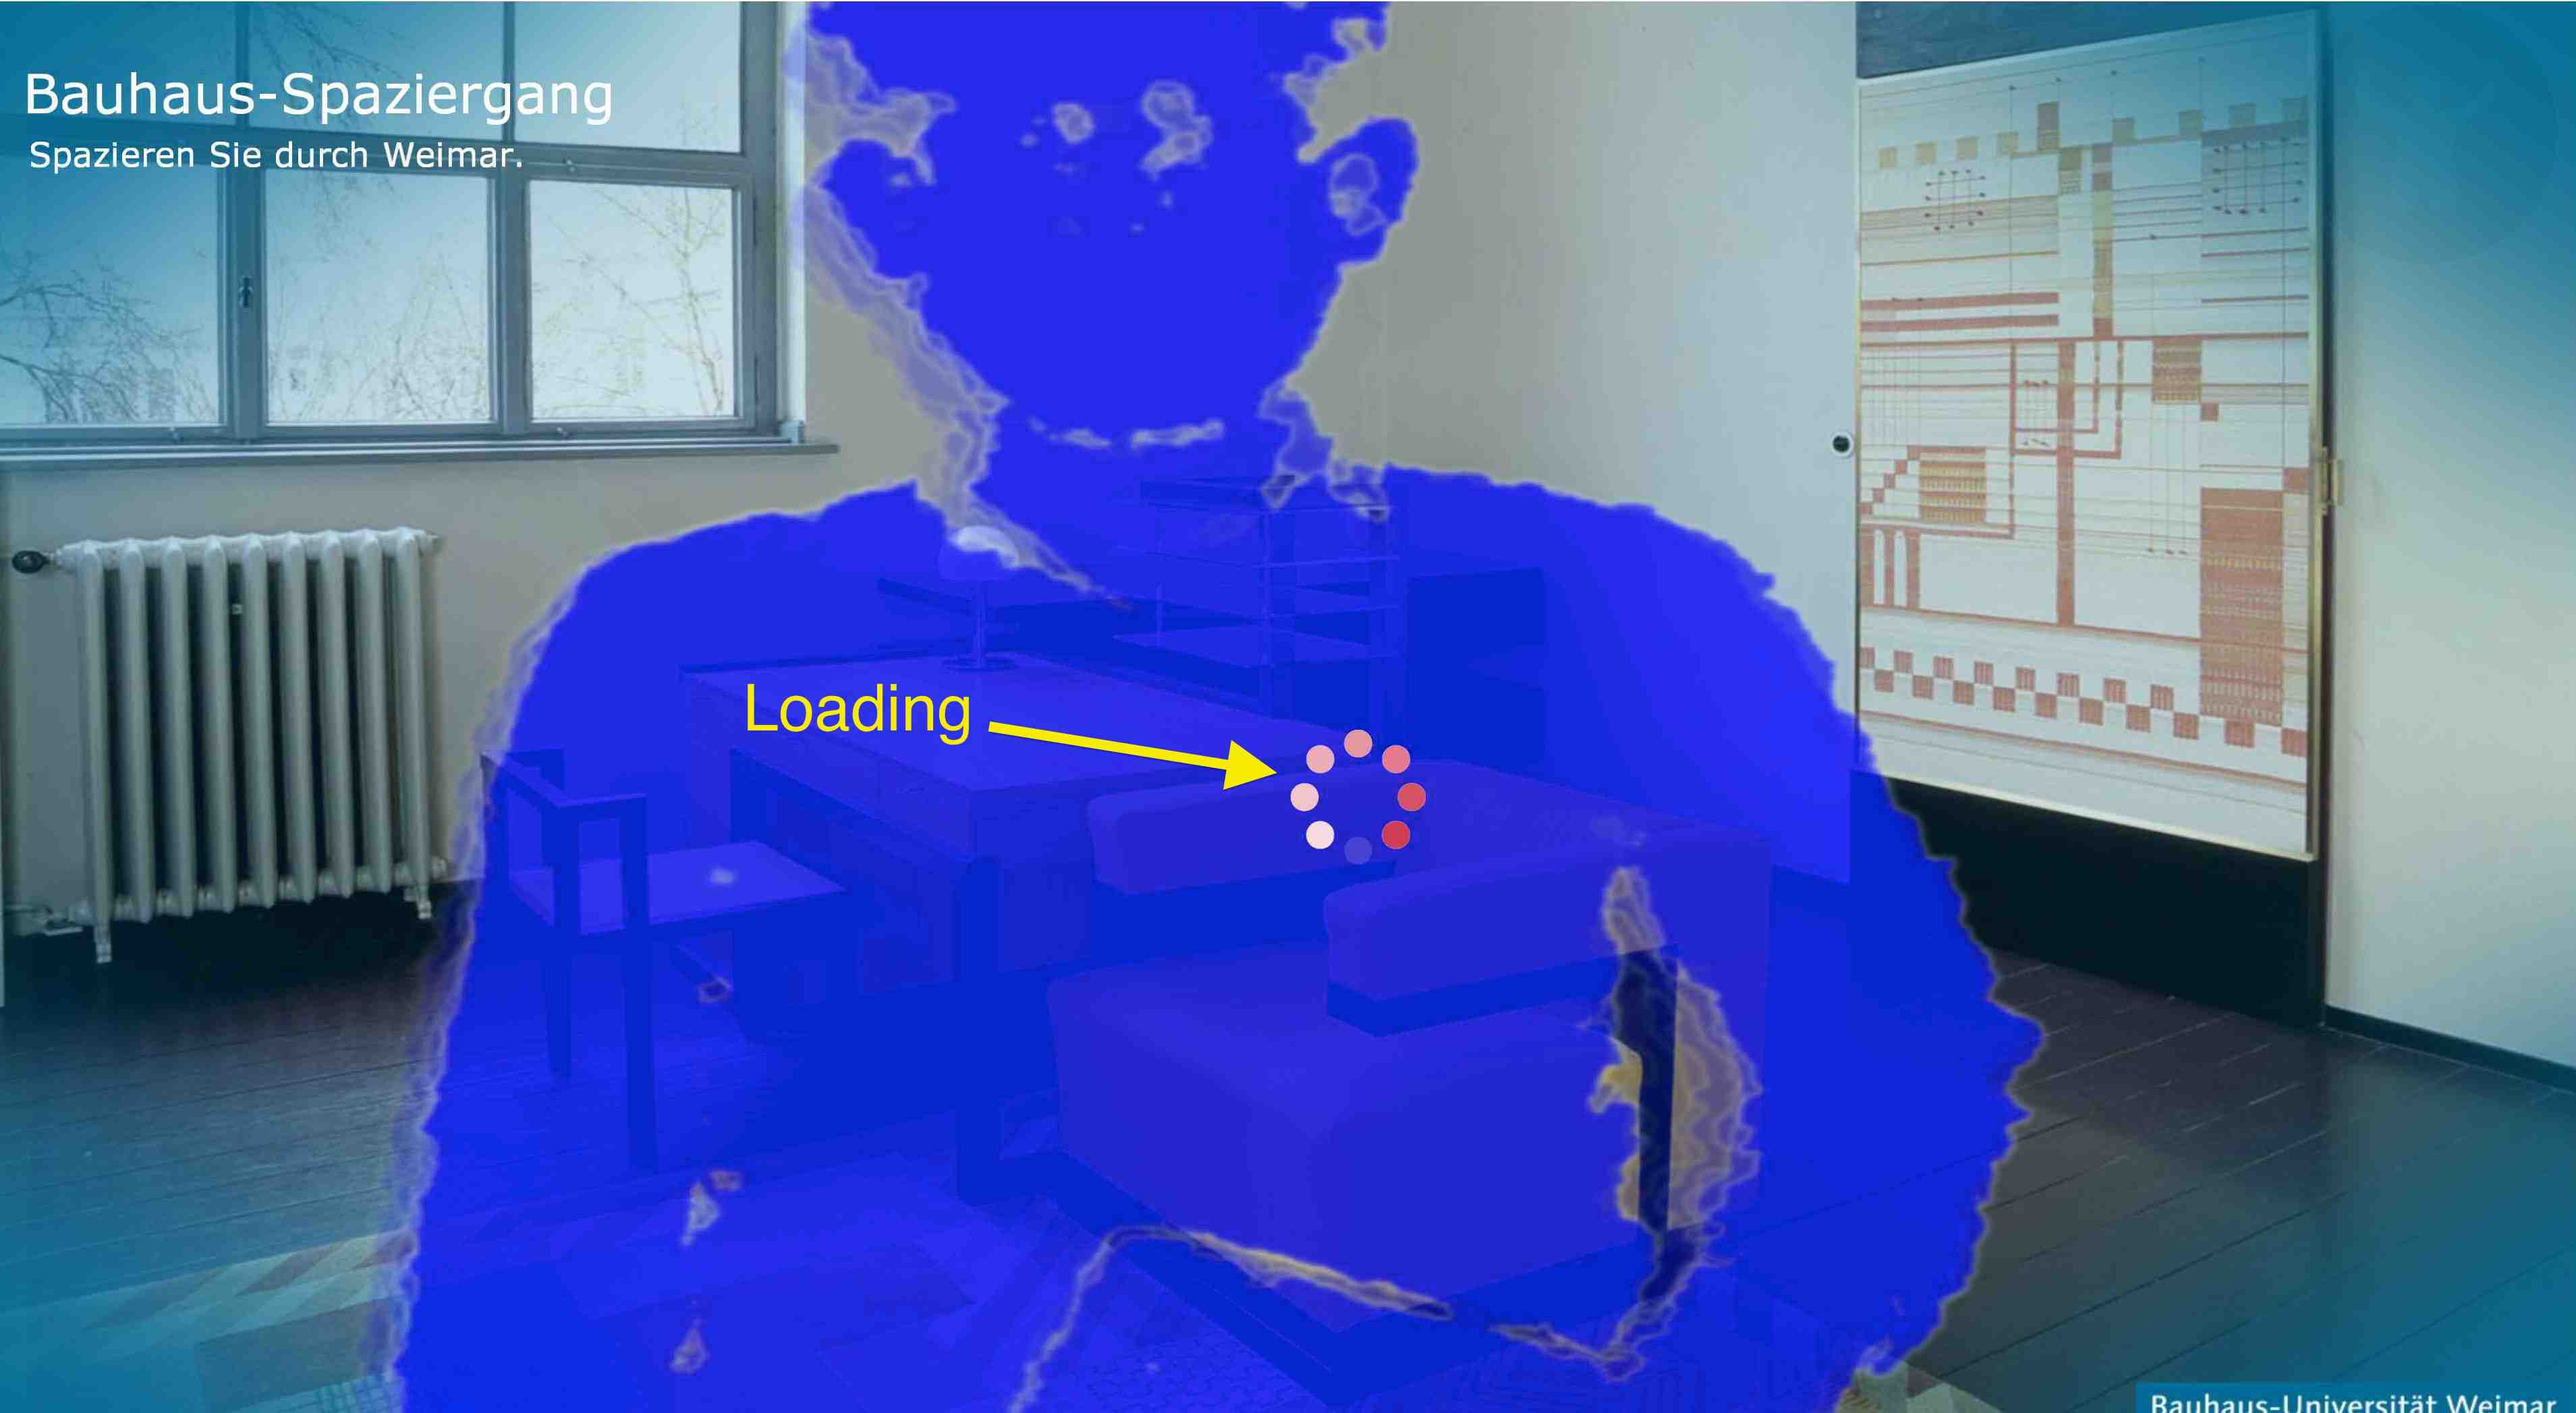
\includegraphics[width=\textwidth,height = 3.5cm]{Figures/7/body_interactive/loading}
        \caption{}
        \label{fig:loading_logo}
    \end{subfigure}
    \begin{subfigure}[H]{0.32\textwidth}
        \centering
        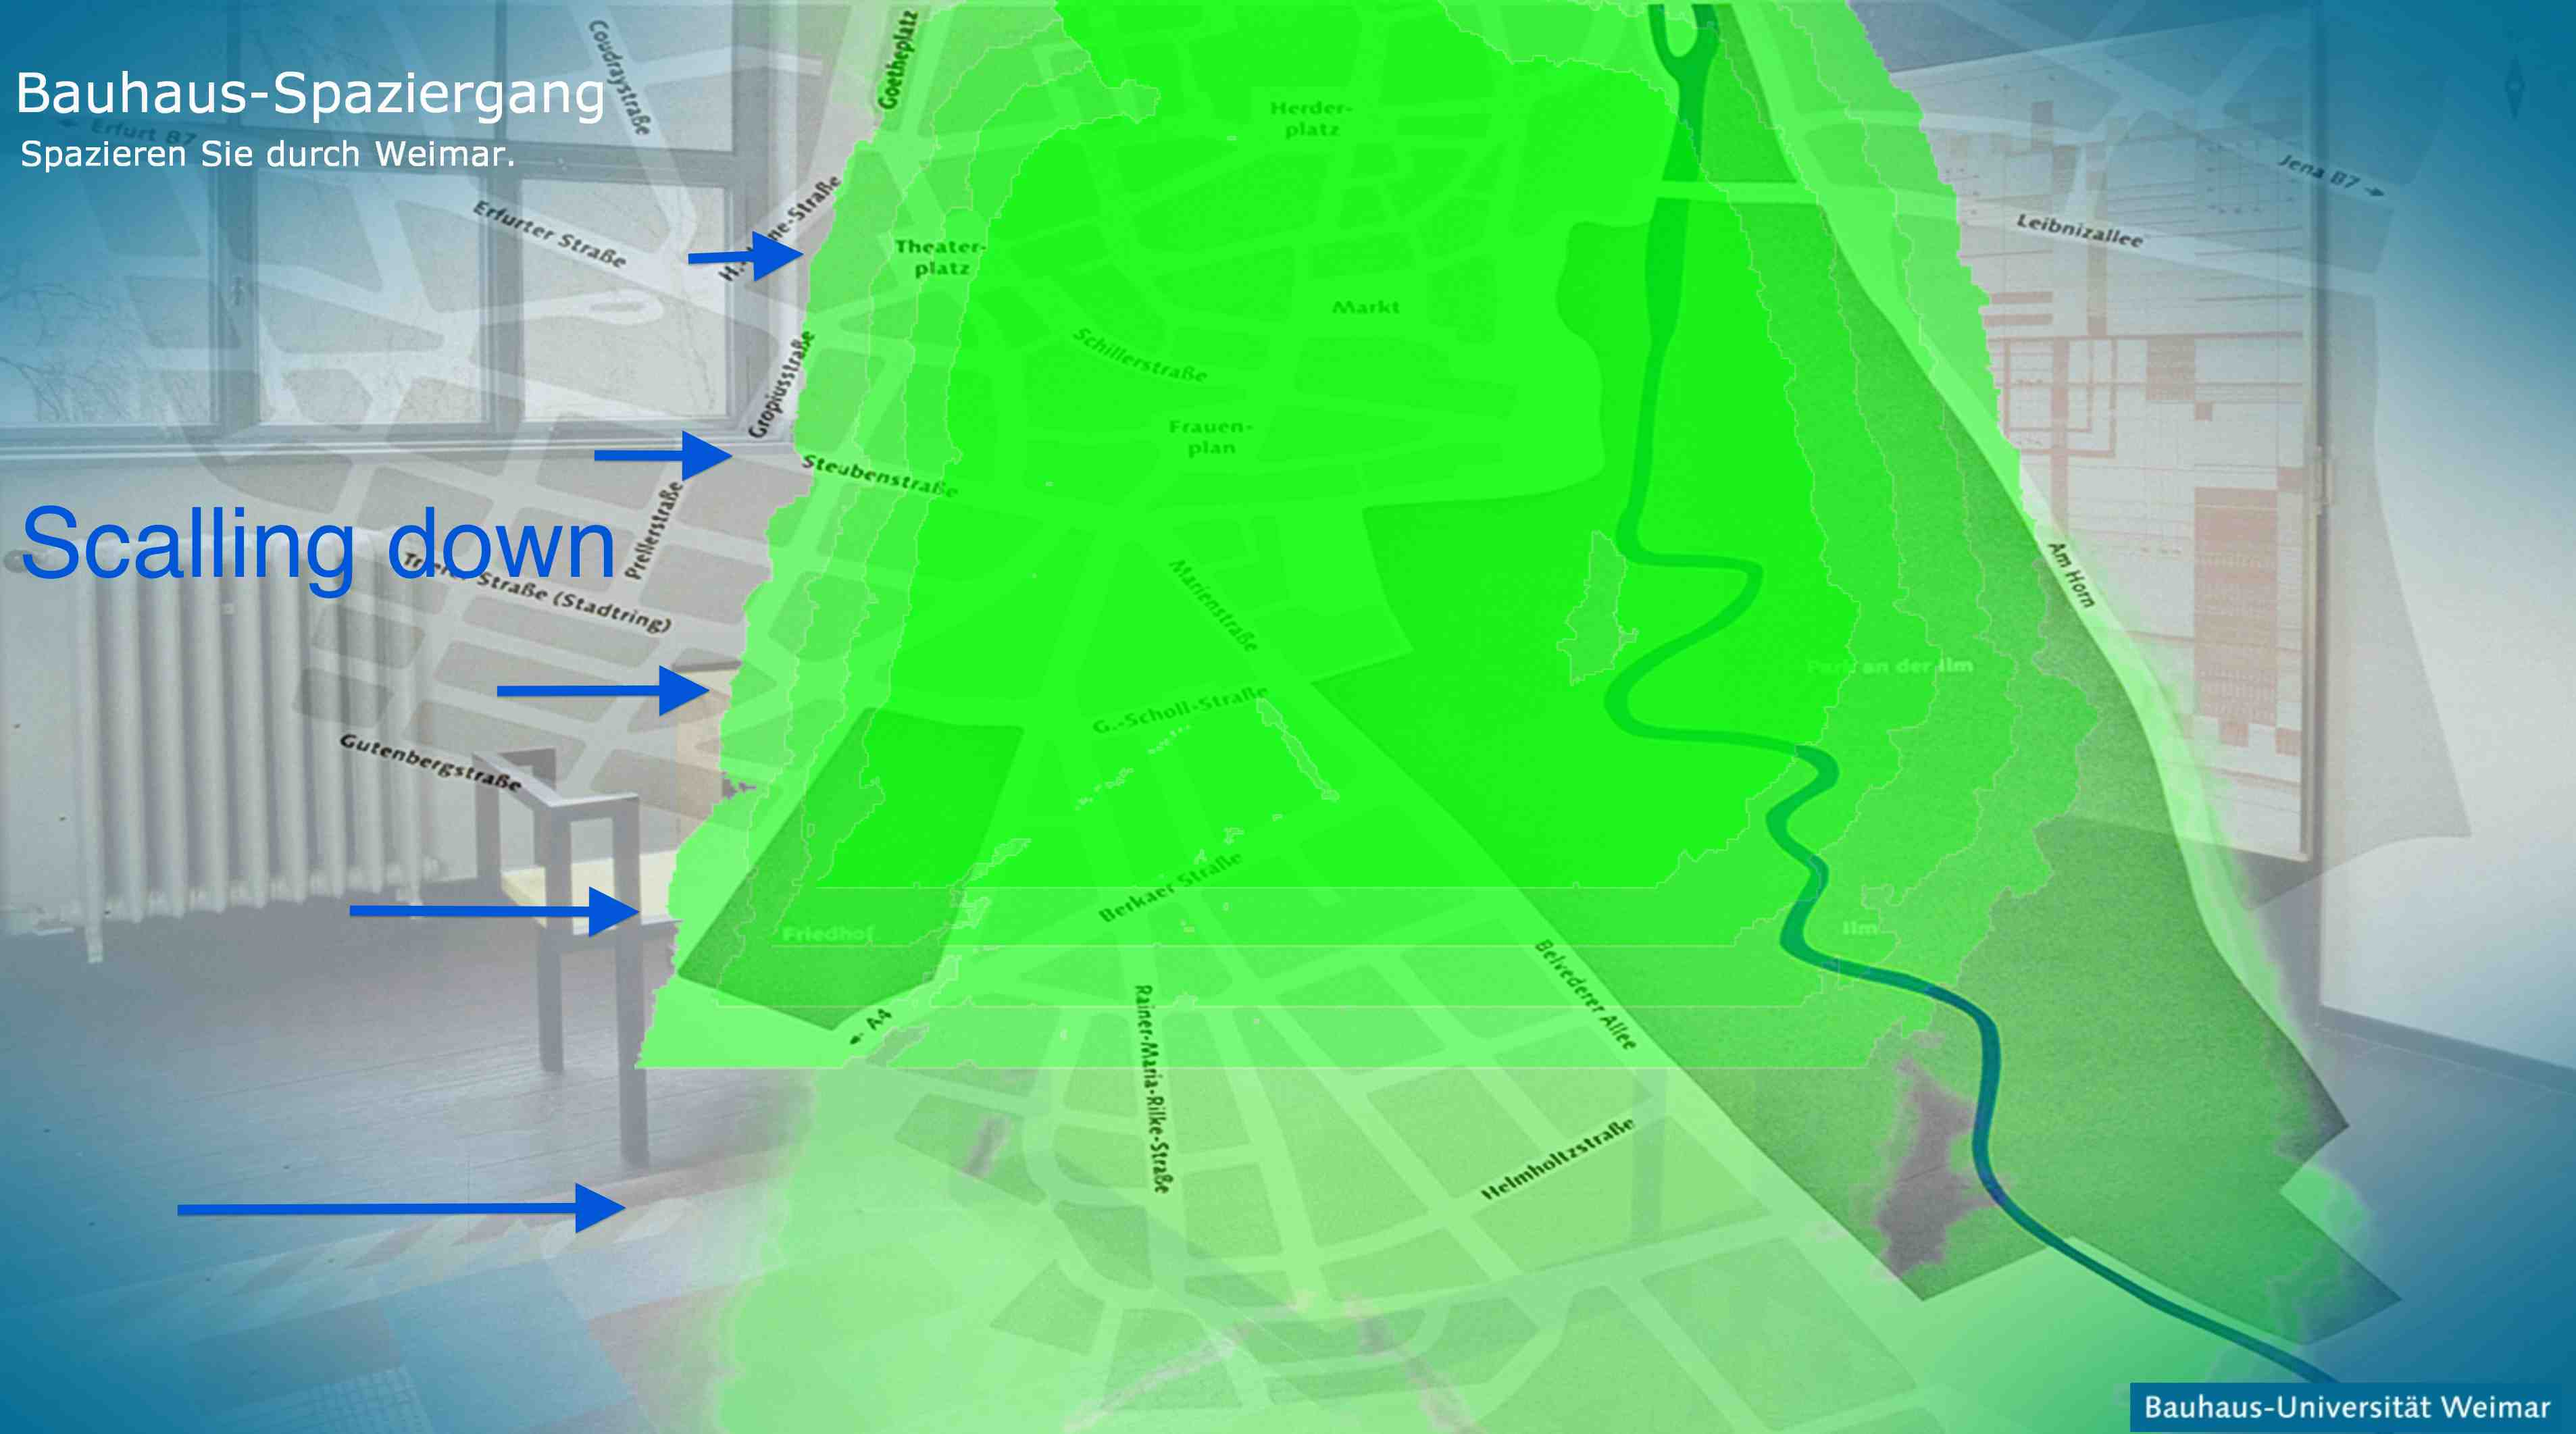
\includegraphics[width=\textwidth,height = 3.5cm]{Figures/7/body_interactive/scalling_down}
        \caption{}
        \label{fig:scalling_down}
    \end{subfigure} 
      \begin{subfigure}[H]{0.32\textwidth}
        \centering
        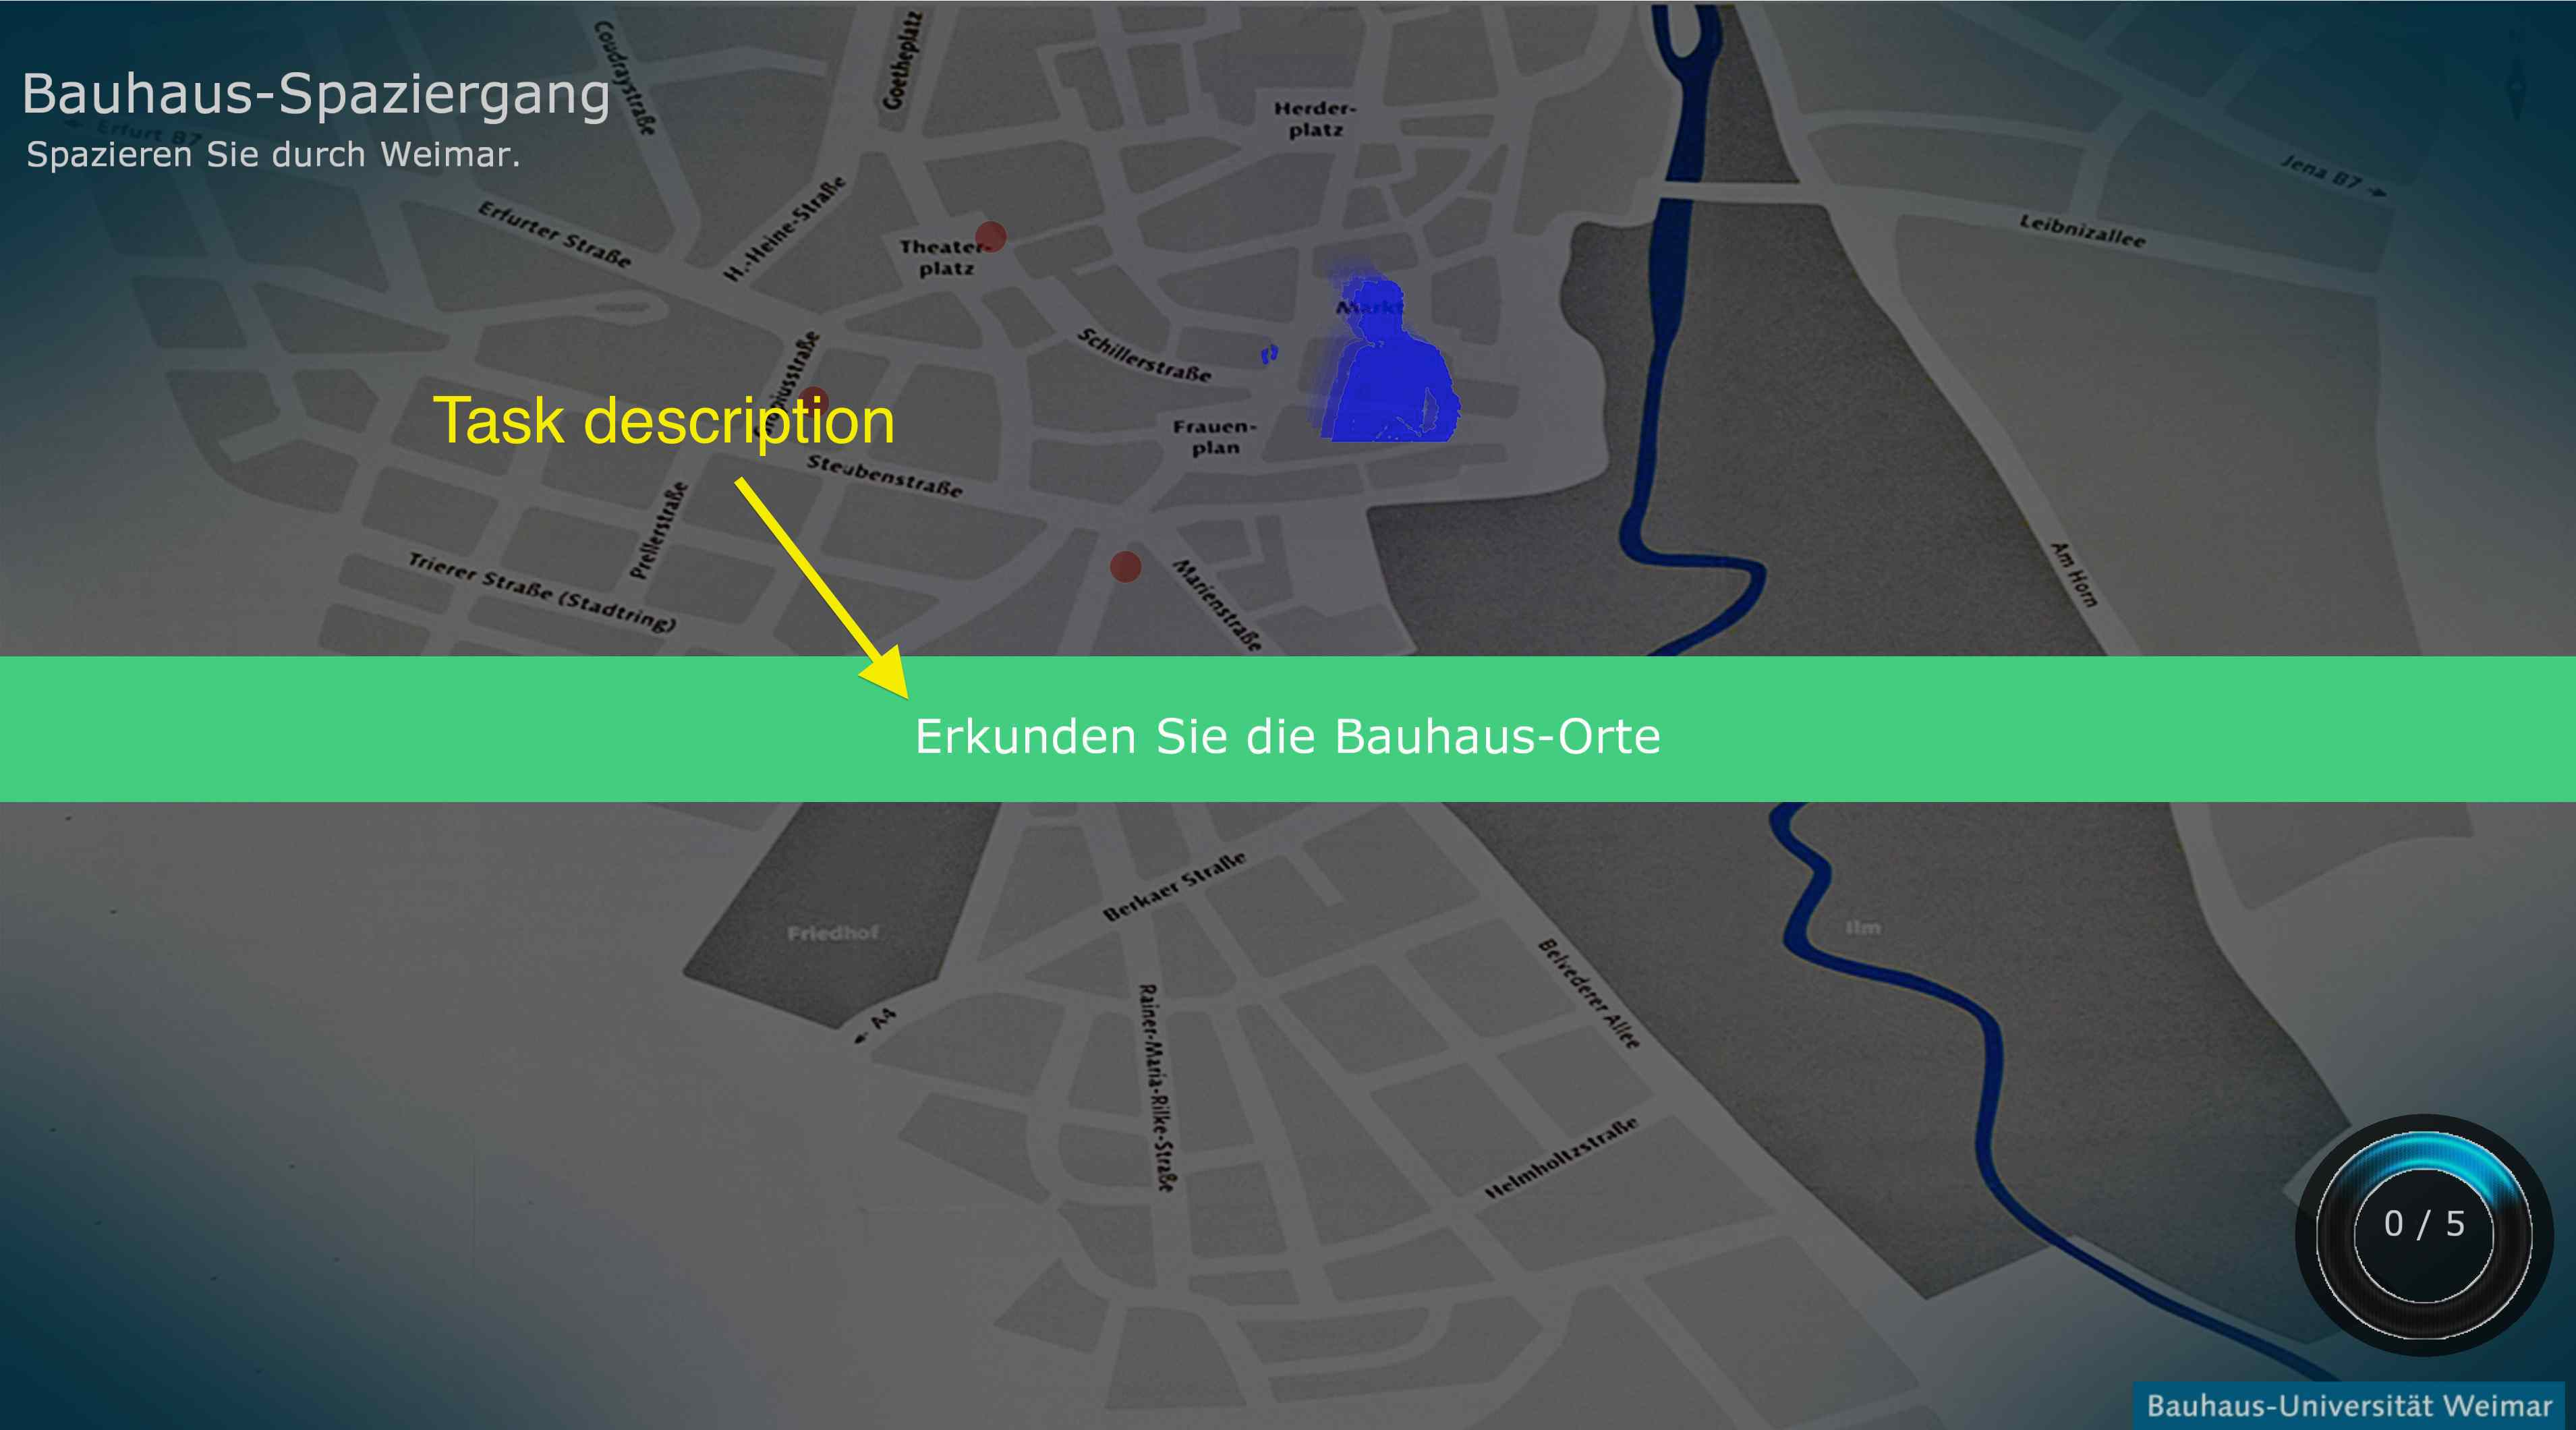
\includegraphics[width=\textwidth,height = 3.5cm]{Figures/7/body_interactive/task_description}
        \caption{}
        \label{fig:task_description}
    \end{subfigure}
    \caption{}
    \label{fig:transition_sequence}
\end{figure}

The picture A shows that the person is close to the screen and the loading of the animation begins. In picture B, the person's silhouette is being scaled down (in this example the silhouette color is green) and in picture C, the instructions are shown.


\item Map Interface (Interaction): \\
In this interface participants can interact with the elements on the map. In the below picture, the silhouette has visited two locations therefor has 2/5 score, to finish the interaction he needs to visit all the location or the timer(40 seconds) on the corner right will be over.\begin{figure}[H]
    \centering
    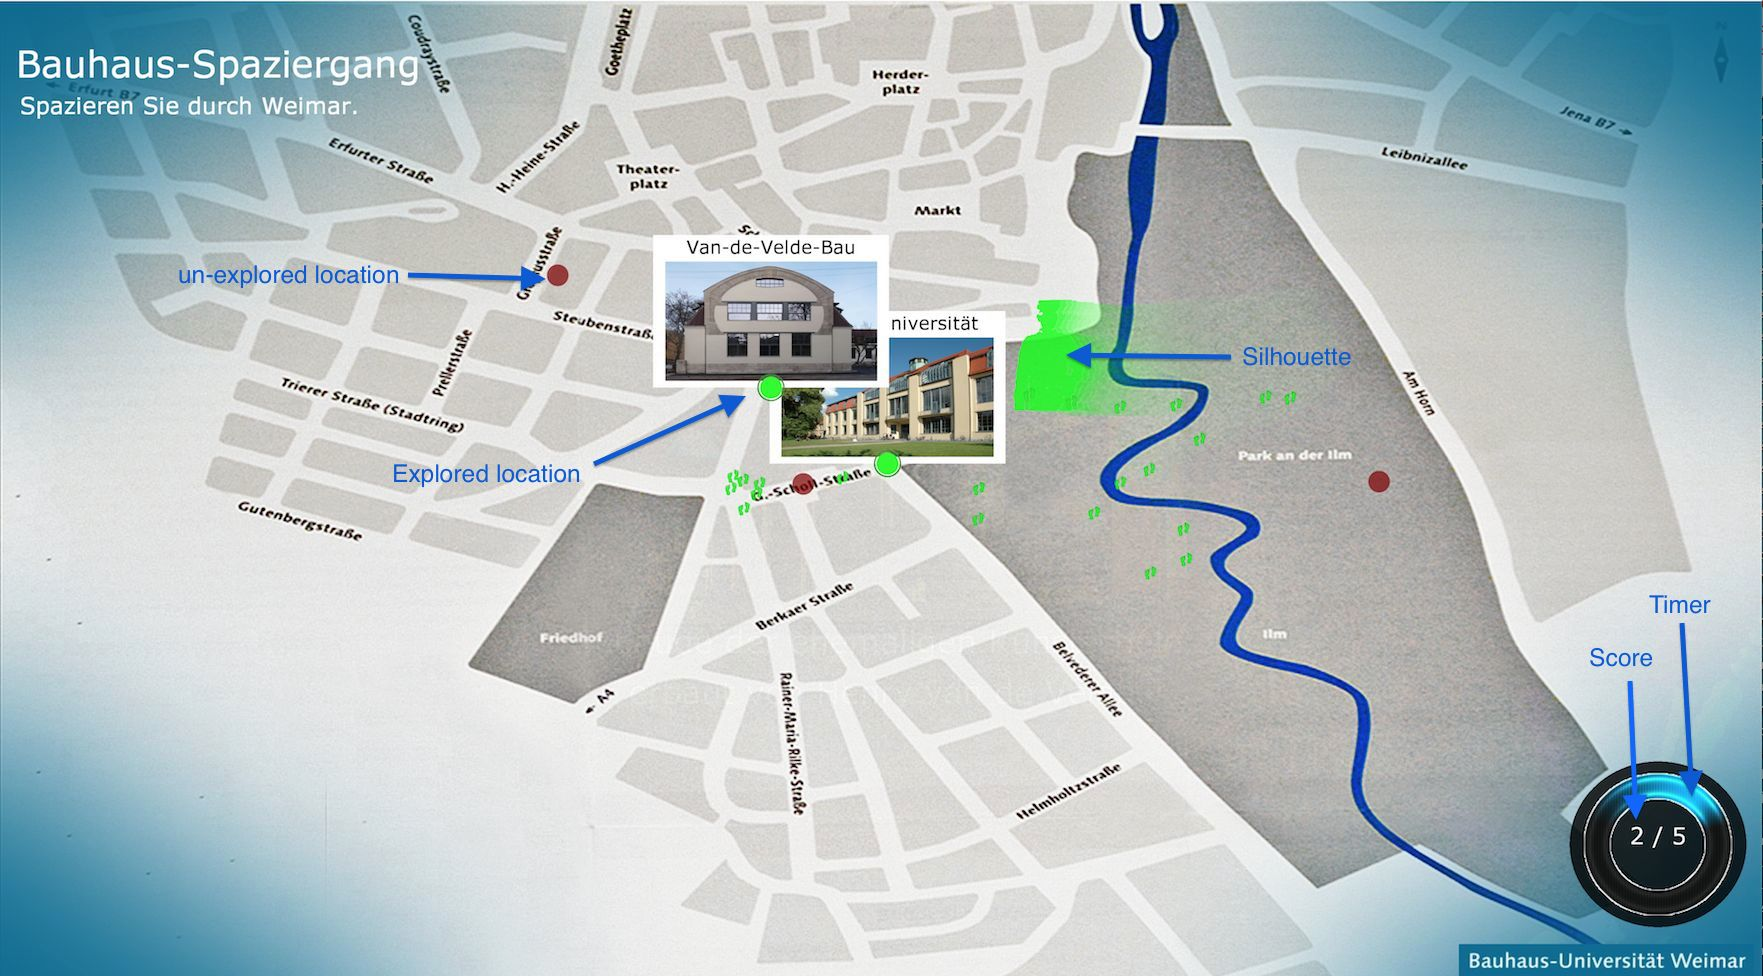
\includegraphics[width=0.8\textwidth,height=70mm]{Figures/7/body_interactive/second_interface}
    \caption{Map Interface}%
    \label{fig:body_secondinterface}%
\end{figure}

\item Advertisement video:\\
The same advertisement video, which was for non-interactive, is shown after the interaction is completed.

\end{enumerate}

\iffalse
\subsubsection{Flowchart Diagram}
The below chart roughly shows the flow of the application.
\begin{figure}[H]
    \centering
    \includegraphics[width=120mm,height=140mm]{Figures/7/body_interactive/body_flow_chart}
    \caption{Body Interactive advertisement Flowchart diagram}%
    \label{fig:Body_flowchat}%
\end{figure}


\subsubsection{Software Details}
The application is developed in Processing language with the support of Kinect Library, The application can run in Windows and OSX operating systems the system should have below requirements.

\begin{itemize}
\item Processing v2.2.2.
\item SimpleOpenNI library for Processing \cite{simpleopenni}
\item 32bit JRE (Java Runtime Environment) v1.8 or higher.
\item Windows / Mac OSX
\item RAM: 4GB or above.
\item CPU: Core i5 / i7 2.3Ghz
\end{itemize}

Refere to source code in DVD that has all the libraries and important things you require to run the application.

\fi

\subsubsection{Mobile Interactive application}
In this application, the display interface is absolutely the same as the other two applications; the only different is that a user carries out the interaction with a smartphone. The mobile interaction technique and platform was adapted from the Bauhaus University \emph{MMM Ball}\cite{MMMball, MMMball2} project under Mobile Media Group\footnote{Mobile Media Group: \url{https://www.uni-weimar.de/de/medien/professuren/mobile-media/}, last accessed 5 jun 2016} department.

\begin{enumerate}

\item Initial Interface (\emph{Call-to-Action}) : \\
This interface is designed in such a way to attract passers-by and also guide the participants on how to use their smartphone to access the advertisement application. The attraction is again the same method that was used for the body, the passers-by silhouette is projected at the back of Access information. The interface has a QR code that could be easily scanned instead of typing the whole IP address. There is an alert area that gets activated when a logged in person has not turned their phone in landscape orientation.
\begin{figure}[H]
    \centering
    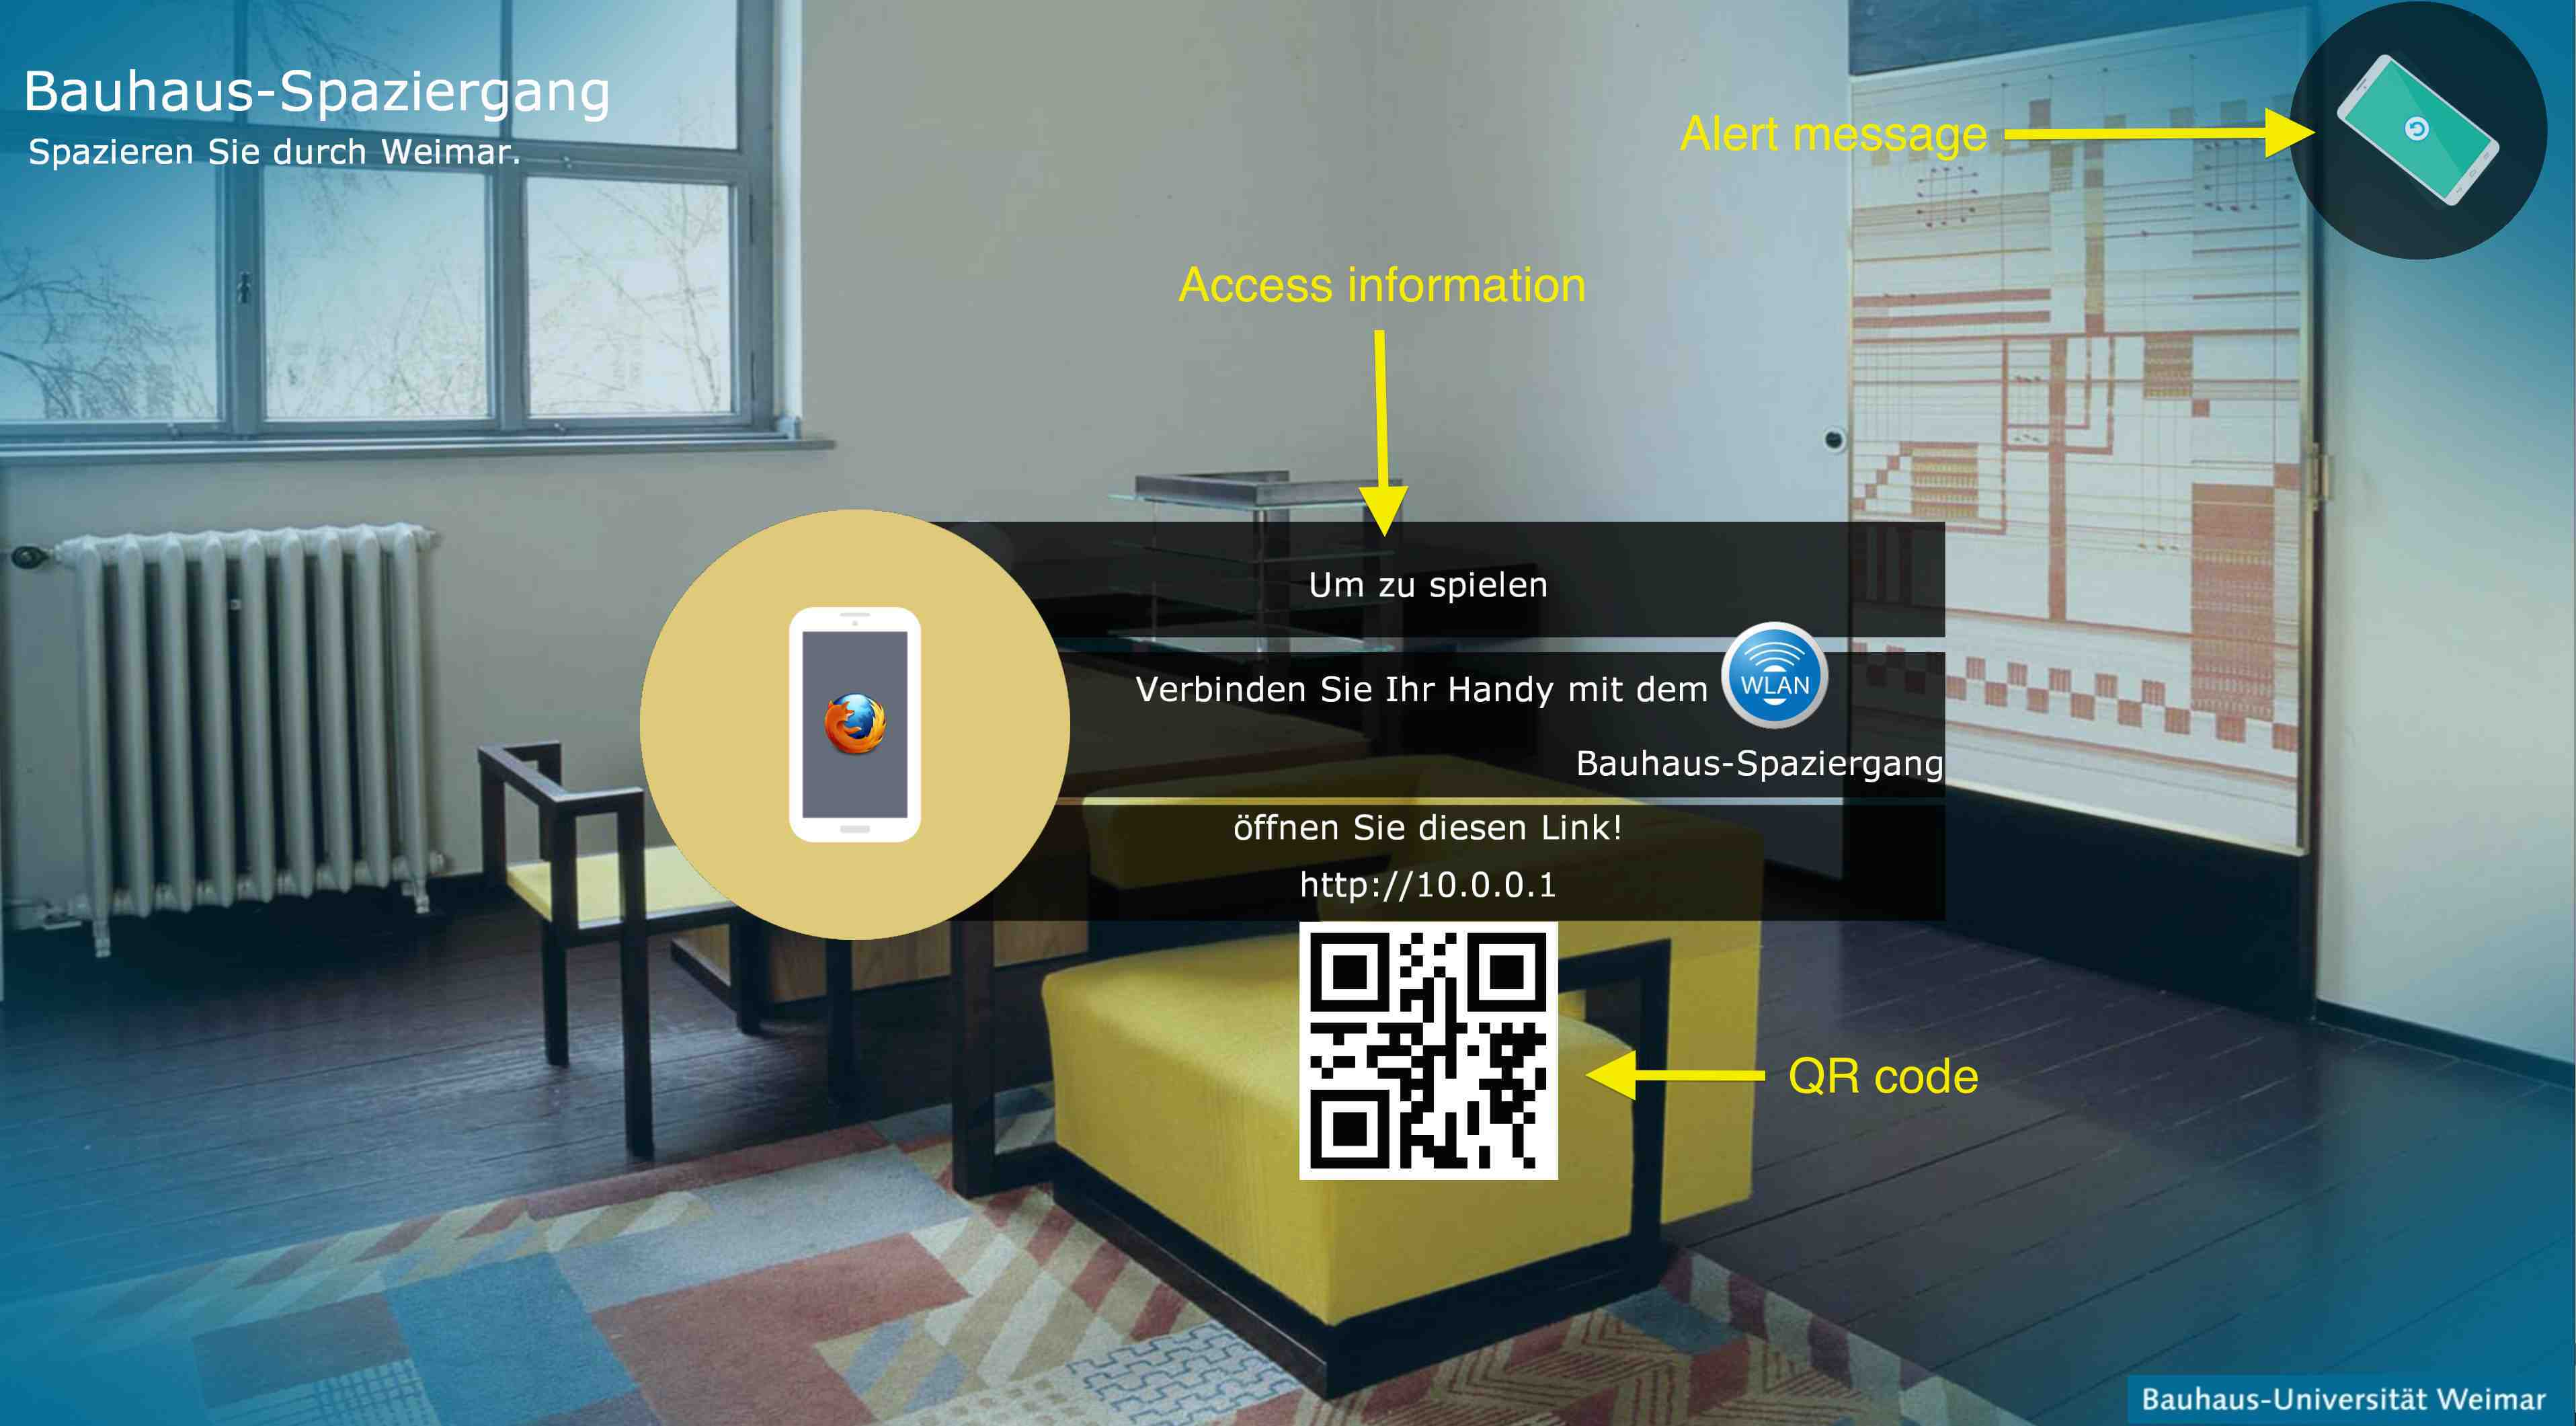
\includegraphics[width=0.8\textwidth,height=70mm]{Figures/7/mobile_interactive/first_interface}
    \caption{Initial Interface}%
    \label{fig:mobile_firstinterface}%
\end{figure}



\item Transition to Map Interface: \\
The user should login to the advertisement system, open the interaction controller, hold the mobile in landscape mode and then the following process will be triggered. 

\begin{enumerate}
\item Loading animation:\\
The loading animation is a reaction to the action of the participants, which gives the user a clue that the interaction will be started. 
\item  Creating Colored cursor: \\
A colored circle will be created for the participant in the center of the screen; each participant would have different colors matching to their controller interface in their phone.
\item Show task instruction:  \\
The instruction is fairly very easy and it is simplified in one sentence to explore locations on the map by using their phone.

\end{enumerate}


\begin{figure}[H]
    \centering
    \begin{subfigure}[H]{0.48\textwidth}
        \centering
        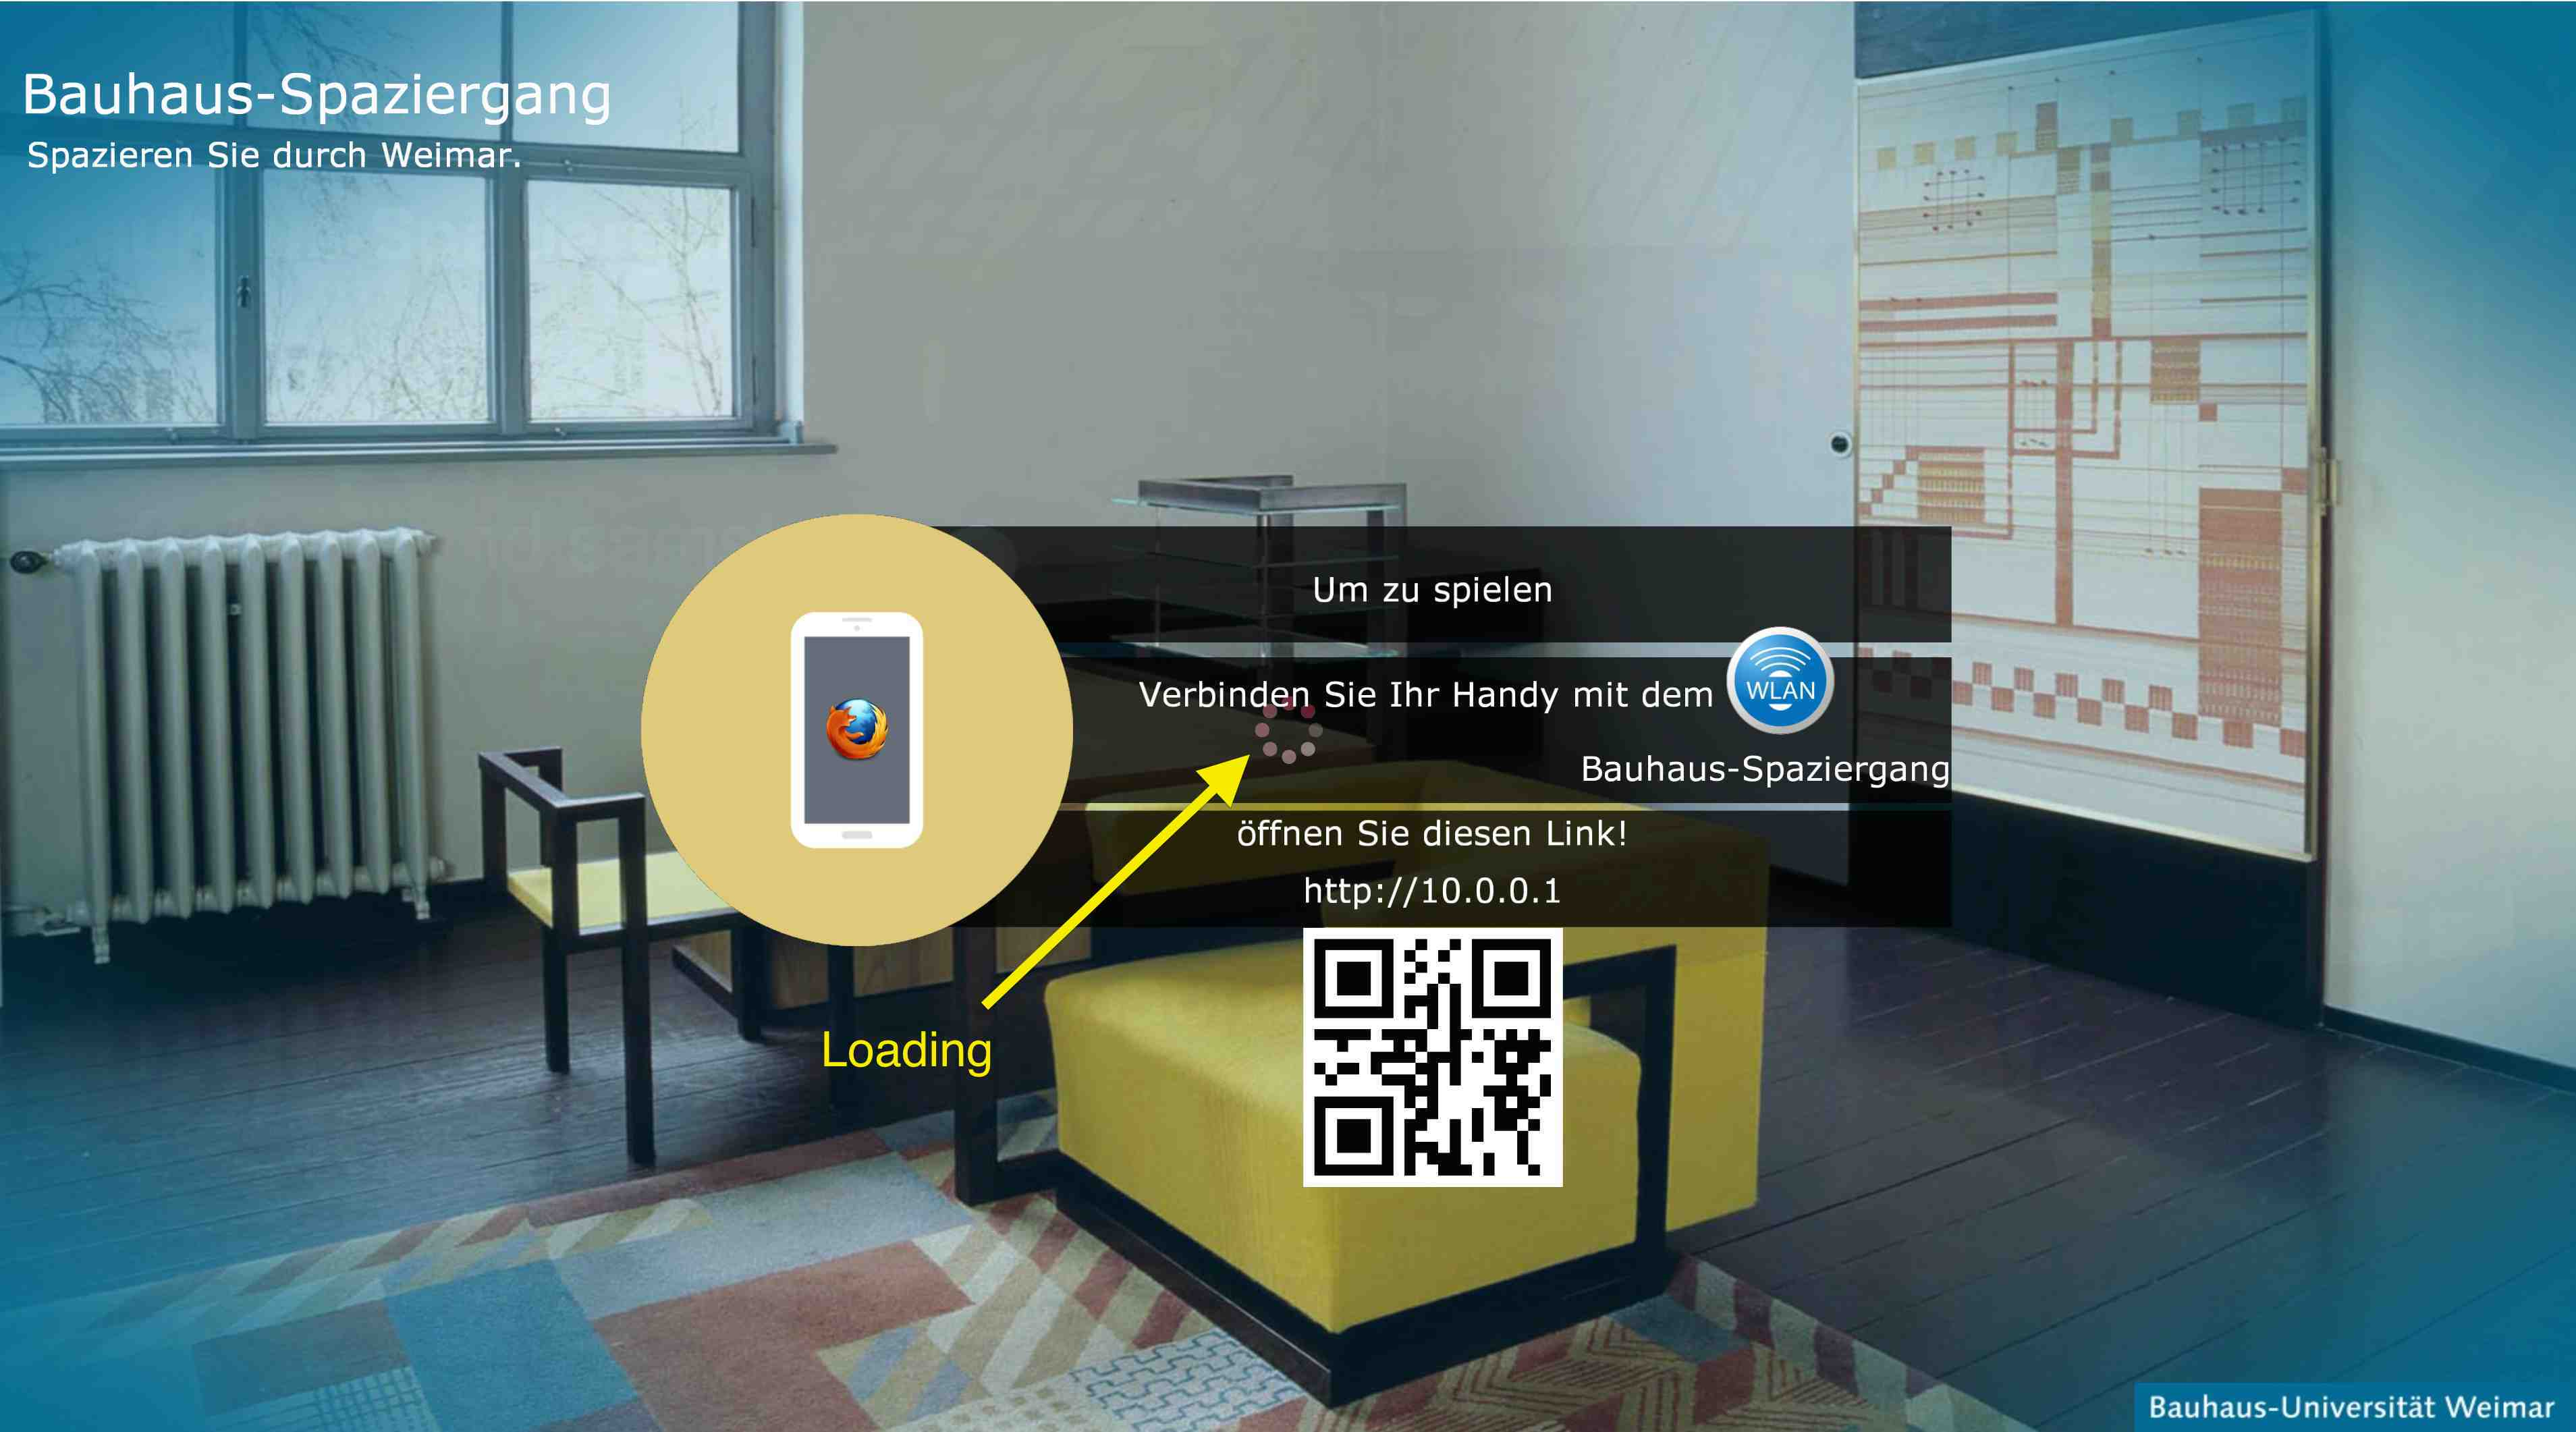
\includegraphics[width=\textwidth,height=5cm]{Figures/7/mobile_interactive/loading}
        \caption{}
        \label{fig:loading_mobile}
    \end{subfigure}
    \begin{subfigure}[H]{0.48\textwidth}
        \centering
        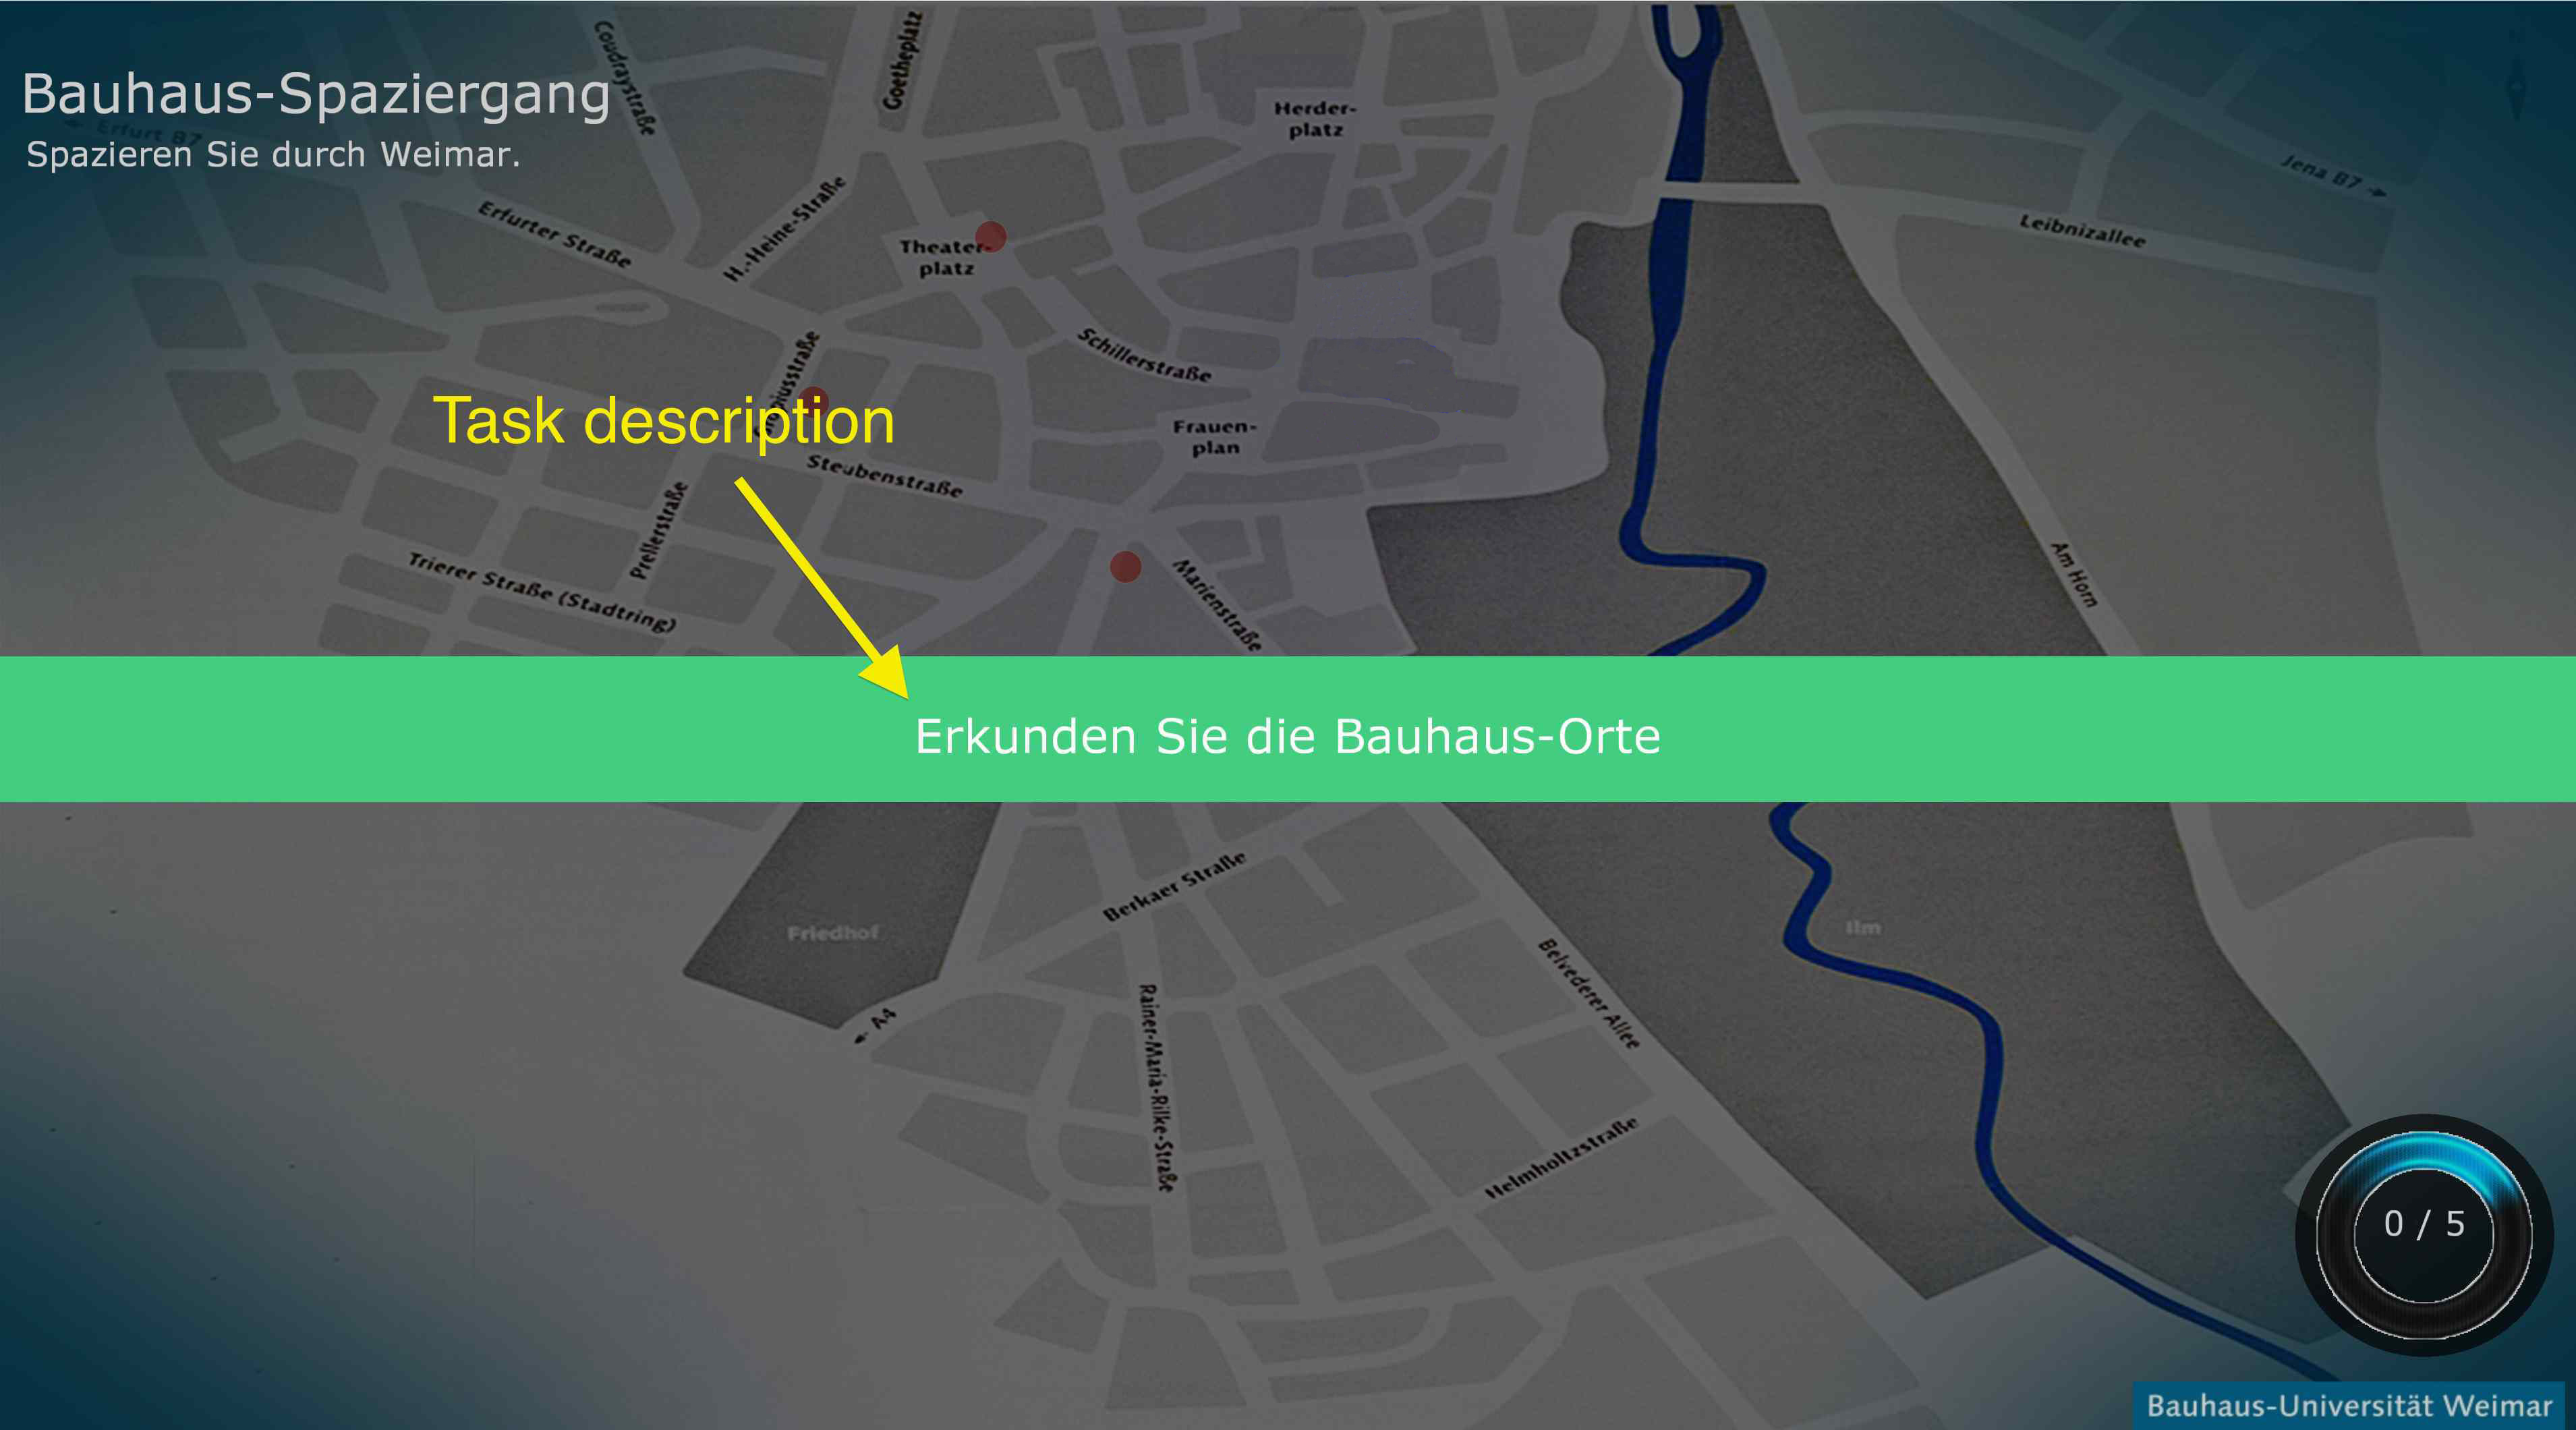
\includegraphics[width=\textwidth,height=5cm]{Figures/7/mobile_interactive/task_description}
        \caption{}
        \label{fig:task_mobile}
    \end{subfigure}
    \caption{Transition of interface}
    \label{fig:Switching_between_phases_mobile}
\end{figure}

In picture (A) a user has logged in and the screen is loading, in picture (B) the task description is shown.


\item Map Interface (Interaction): \\
This interface is where the users interact with the map; participants can navigate using the controller page on their phones. The image \ref{fig:mobile_secondinterface} displays that the user is controlling the cursor and has explored one location. The user's defined login name is also shown on the cursor to provide a hint that he/she is his circle. To reach an interest point a small circle is shown to determine the area of intersection. The interaction finishes when all the locations are explored or the interaction time (40 seconds) gets over.


\begin{figure}[H]
    \centering
    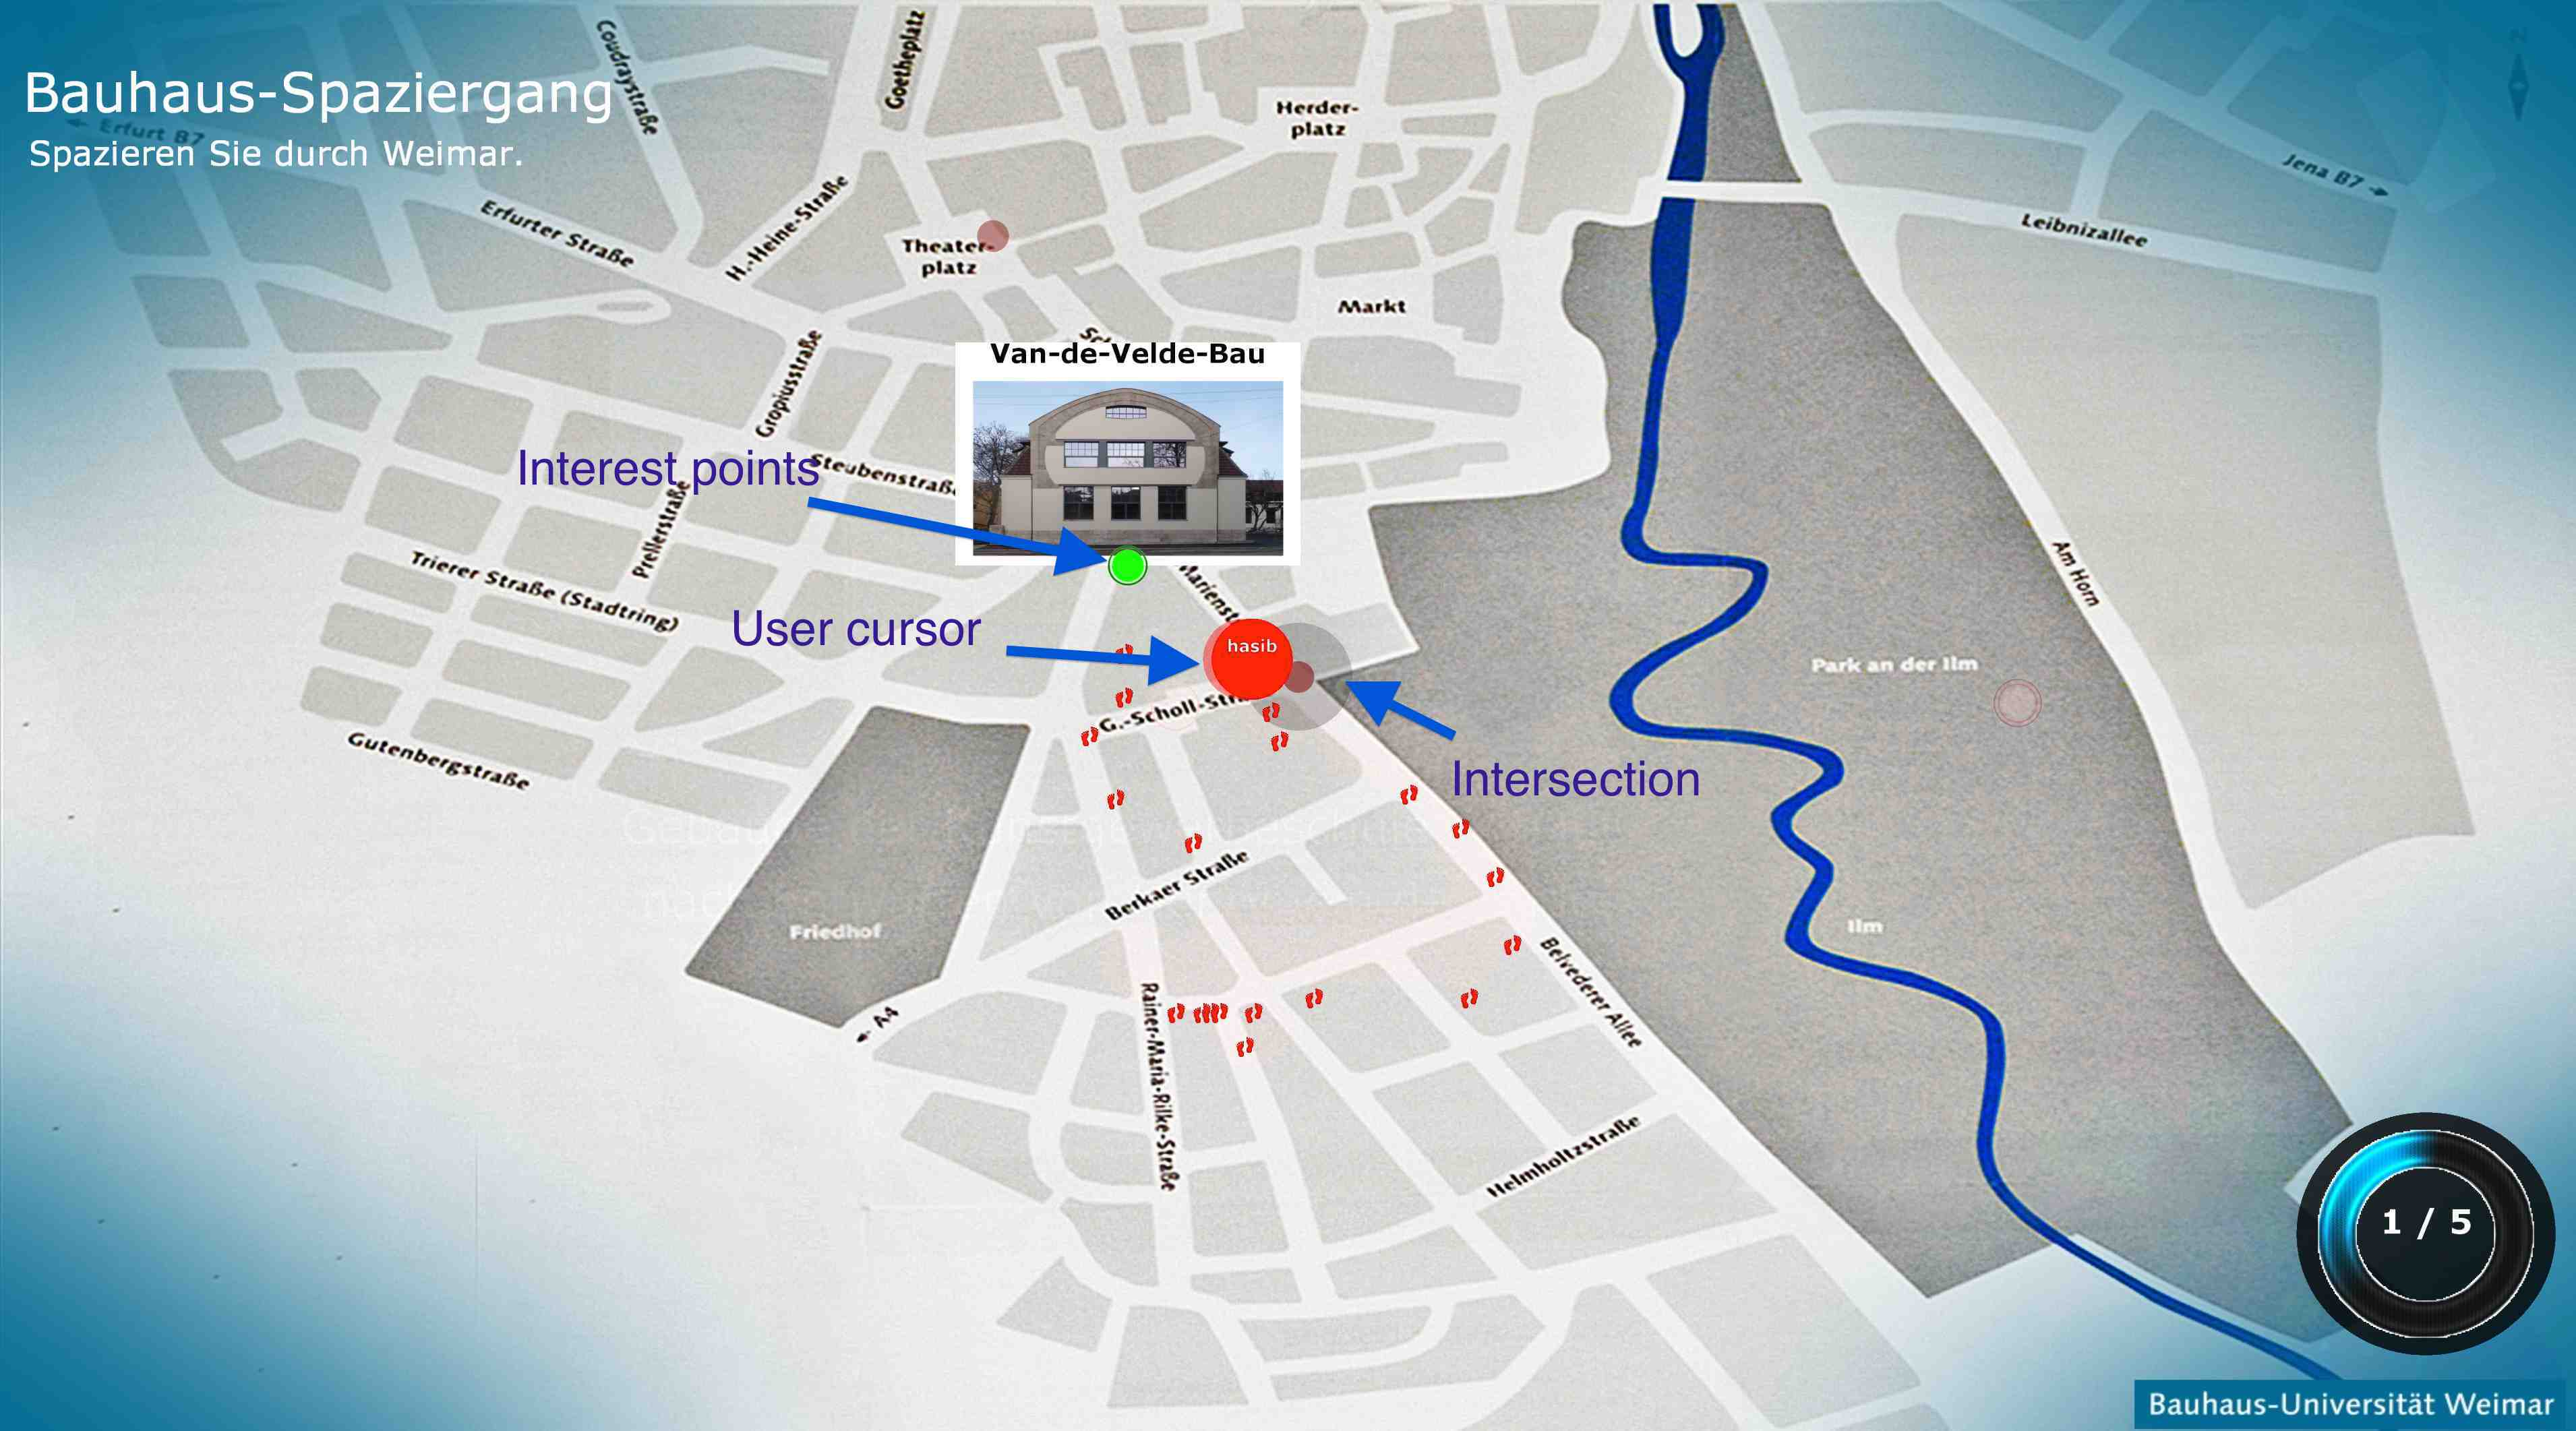
\includegraphics[width=0.8\textwidth,height=70mm]{Figures/7/mobile_interactive/second_interface}
    \caption{Map interface}%
    \label{fig:mobile_secondinterface}%
\end{figure}

\item Advertisement video:\\
The same advertisement video used for non-interactive is shown after the interaction is completed.


\item Mobile interface: \\
The interaction controller in the smartphone is shown below. The interface is very simply designed and has two elements, the cursor and the select button. With the cursor, the user can navigate inside the map to interest points and on reaching on an interest point the participant presses the select button to explore that location. 

\begin{figure}[H]
    \centering
    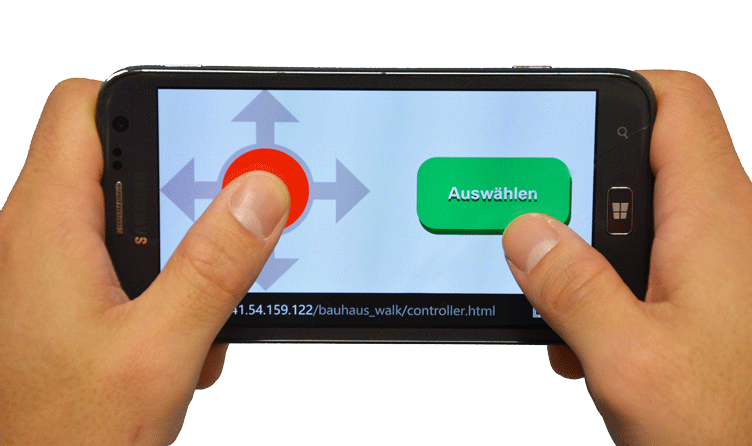
\includegraphics[width=100mm,height=60mm]{Figures/7/mobile_interactive/mobile_interface}
    \caption{Mobile controller}%
    \label{fig:mobile_controllerinterface}%
\end{figure}

\end{enumerate}

\iffalse

\subsubsection{Hardware setup}
The hardware required for the type of interactive application, would be to use one Access point that enable participants to connect to the system, Kinect camera to record colored user images, a mobile phone at client side and obviously the screen and a workstation.


\begin{figure}[H]
    \centering
    \includegraphics[width=100mm,height=60mm]{Figures/7/mobile_interactive/Mobile_hardware_setup}
    \caption{Hardware setup}%
    \label{fig:mobile_hardware_setup}%
\end{figure}


\subsubsection{Software setup}
In order to make the system running we would need the below things.
\hilight{The controller is taken from another project MMM ball}
\begin{itemize}
\item Apache webserver:\\
The web server could be running in the same application system side-by-side. The web controller is using WebSocket client at the backend. Check the JavaScript configuration
file to have the IP address configured where application system is using.
\item Processing and WebSocket:\\
The application should be started and along that the WebSocket server should also be running silmultaniously. Processing should have WebSocket library installed before hand. The system should have a valid IP address to be reached by webserver.
\item OpenProcessing Library:\\
Processing should have OpenProcessing library installed to be able to run Kinect Camera for color image recording.
\end{itemize}


\begin{figure}[H]
    \centering
    \includegraphics[width=120mm,height=60mm]{Figures/7/mobile_interactive/mobile_software}
    \caption{System architecture}%
    \label{fig:mobile_software_setup}%
\end{figure}

To have a full look to the software, please refer to the DVD to see all the source codes and the relavent applications.

\subsubsection{Flowchart Diagram}
The below chart roughly shows the flow of the application.
\begin{figure}[H]
    \centering
    \includegraphics[width=130mm,height=160mm]{Figures/7/mobile_interactive/mobile_flow_chart}
    \caption{Mobile Interactive advertisement Flowchart diagram}%
    \label{fig:mobile_flowchat}%
\end{figure}
\fi

\section{Interaction Design}
The body interaction model is designed based on \emph{Audience funnel},  a it suites well for public setups like the Tourist information center and advertising. With the design of this interaction model different levels of interactions and phases can be observed. Based on this model the three phases of the applications were designed (\emph{Call-to-Action}, Interaction interface and ad video). This model attracts passersby and gradually motivates them toward the display to engage them in interaction and at the same time it is also convenient for the passers-by to avoid the display


\subsection{Body Interaction Design}
The diagram below shows the display at the top, the body-tracking area illustrated by a triangle. This triangle is divided into two sections that is separated by dashed lines, (1) gray region defines the least interest regions, because in this area it is assumed that people maybe busy with other things around the display, and people in this region can easily avoid the display and the display will not motivate them for interaction, and (2) the highest interest region, it is assumed that people are aware of the display and the display would motivate them for interactions only if they are facing towards display.


\begin{figure}[H]
    \centering
    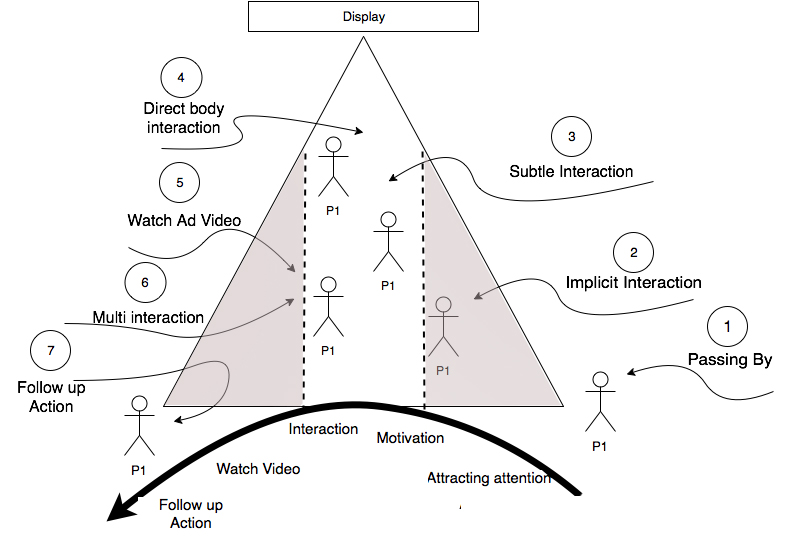
\includegraphics[width=0.9\textwidth,height=8cm]{Figures/7/body_interaction_model}
    \caption{Body interaction design.}%
    \label{fig:body_interaction_deisng}%
\end{figure}


The model consists of seven phases, each of them are explain in the following list.

\begin{enumerate}
\item \emph{Passing by phase:} \\
This phase demonstrates passersby, who are not in the display tracking range.

\item \emph{Implicit Interaction phase:} \\
This phase starts, when passersby are in tracking range but are standing far or at side of the display. 

\item \emph{Subtle interaction phase:} \\
In this phase, the user is in near or center area of tracking range and facing toward display. The system motivates the user for direction interaction with the \emph{Call-to-Action} feature (``\emph{To play, Come near}'').

\item \emph{Direct body interaction phase:} \\
This phase happens, when the user has actively started the game interaction and is playing. At this phase the whole tracking range (gray and white color) could be used for direct interaction until the end of interaction phase.

\item \emph{Watch ad video phase:} \\
When the interaction is over, a short advertisement video is shown.

\item \emph{Multi interaction phase:} \\
This phase demonstrates that the user can perform interaction multiple times.

\item \emph{Follow up action phase:} \\
Follow up action phase is, when the user leaves the display’s tracking range and performs other actions.

\end{enumerate}


The Black curve below the diagram shows the transition of the user between each phase and shows the flow of the attention, motivation, interaction and other phases. The attention is captured mainly in \emph{Implicit interaction phase}, the motivation occurs when the user is in \emph{Subtle interaction phase} and the interaction is when the user is directly playing with the his/her silhouette in the entire tracking coverage area. After the interaction and watching ad video, the curve changes direction moving down, which illustrates that the user would likely leave the interaction area and follow other actions unrelated to the screen. 

\begin{itemize}

\item Attention: \\
A \emph{Bottom-Up} approach was used to achieve the passers-by attention because the approach can help get attention by showing a sudden object, or by contrasting various colors. To do so, the silhouette representation of passers-by were projected on the screen, this representation can bring higher level of attraction as it is responsive to the user movements, and has different contrast colors in relation to background. In chapter 3, this method was compared with other forms of representation and attracting attention and the silhouette was the top candidate.

\item Motivation: \\
The motivation is done by bring joy, fun, curiosity and challenge\cite{ toward_motivation} to the users who are attracted toward thedisplay. In body interaction design the use of passers-by’s silhouette presentation would be a good motivational force to bring passers-by near the display. This technique can become a source of fun and entertainment and can give a sense of connectedness with the display. And at the same time it also motivates passersby by showing a \emph{Call-to-Action} message like “to play! Come near”, which is responsive to user movement and gives them confidence to play.

\item Interaction and follow up actions: \\
When the user starts the interaction, the interaction being carried out should be meaningful, understandable and easy, else the user will leave immediately after some tries. Therefore many focus groups and evaluations of many prototypes were conducted to assure the usability of the body interaction. The interaction is explained in detail in the previous sections.
After the end of the interaction, the advertisement video is shown and then the user can start again interaction or leave the screen.
\end{itemize}


\subsection{Mobile Interaction Design}
Below diagram shows the mobile interaction design. The diagram shows the display at the top, and the triangle represents body-tracking range for passersby. The design has the same 8 phases as proposed for the body interaction. (1) Passing by phase, which demonstrates passers-by who are not in display tracking range, (2) Implicit Interaction phase, the mobile version also has the implicit body interaction for attracting attention only and it is not limited to a certain region, but the whole the tracking area could be used for this purpose, and no further direct interaction is possible, (3) Read Access info, after the user is attracted toward the screen, the user reads how to use his/her mobile phone to connect to the display, (4) connect to system, in this phase the user connects to Wi-Fi and opens the controller, (5) direct interaction phase, is when the user actively interacts using smartphone with the display, (6) Watch ad video, this phase is triggered when the interaction is over, (7) multi interaction phase, demonstrates that the user can perform interaction multiple times, (8) Follow up action phase, is when the user leaves the display’s tracking range and performs other actions.

\begin{figure}[H]
    \centering
    \includegraphics[width=0.9\textwidth,height=8cm]{Figures/7/mobile_interaction_design.png}
    \caption{Body interaction design.}%
    \label{fig:body_interaction_deisng}%
\end{figure}


\begin{enumerate}

\item Attention: \\
Technologies like Bluetooth, infrared and NFC\footnote{NFC: Near Field Communication} of mobile devices in fact could be used for attracting attention of passersby, but these technologies have their limitations and limited usage and not all mobile phones support all of the technologies. At the same time it is possible that the passers-by have not switched on these technologies because of battery consumption or other purpose. Therefore to attract all the passers-by without any limitation, the silhouette representation was used as it was used for body interaction design.

\item Motivation: \\
The motivation is also similar to the body interaction. Due to the display of the silhouette, it brings curiosity and joy to the users. Besides that, an Information text is shown on the screen to give sufficient information on how to access the advertisement system and play the game.

\item Interaction and follow up actions: \\
The interaction with the game element is only possible with the use of a smart phone. The interaction usability is important in order to keep the passersby engaged with the display. Therefore two prototype versions of the mobile interactions were evaluated to remove any possible usability issue. After the interaction is over the advertisement video and other following up action is taken on user.


\end{enumerate}















